\documentclass[12pt,a4paper,twoside,openright]{report}
\let\openright=\cleardoublepage



%%% Choose a language %%%

\newif\ifEN
% \ENtrue   % uncomment this for english
\ENfalse   % uncomment this for czech

%%% Configuration of the title page %%%

\def\ThesisTitleStyle{mff} % MFF style
%\def\ThesisTitleStyle{cuni} % uncomment for old-style with cuni.cz logo
%\def\ThesisTitleStyle{natur} % uncomment for nature faculty logo

\def\UKFaculty{Faculty of Mathematics and Physics}
%\def\UKFaculty{Faculty of Science}

\def\UKName{Charles University in Prague} % this is not used in the "mff" style

% Thesis type names, as used in several places in the title
\def\ThesisTypeTitle{\ifEN BACHELOR THESIS \else BAKALÁŘSKÁ PRÁCE \fi}
%\def\ThesisTypeTitle{\ifEN MASTER THESIS \else DIPLOMOVÁ PRÁCE \fi}
%\def\ThesisTypeTitle{\ifEN RIGOROUS THESIS \else RIGORÓZNÍ PRÁCE \fi}
%\def\ThesisTypeTitle{\ifEN DOCTORAL THESIS \else DISERTAČNÍ PRÁCE \fi}
\def\ThesisGenitive{\ifEN bachelor \else bakalářské \fi}
%\def\ThesisGenitive{\ifEN master \else diplomové \fi}
%\def\ThesisGenitive{\ifEN rigorous \else rigorózní \fi}
%\def\ThesisGenitive{\ifEN doctoral \else disertační \fi}
\def\ThesisAccusative{\ifEN bachelor \else bakalářskou \fi}
%\def\ThesisAccusative{\ifEN master \else diplomovou \fi}
%\def\ThesisAccusative{\ifEN rigorous \else rigorózní \fi}
%\def\ThesisAccusative{\ifEN doctoral \else disertační \fi}



%%% Fill in your details %%%

% (Note: \xxx is a "ToDo label" which makes the unfilled visible. Remove it.)
\def\ThesisTitle{Optimalizace rozmístění stanic pro nabíjení elektrických vozidel}
\def\ThesisAuthor{David Beinhauer}
\def\YearSubmitted{2022}

% department assigned to the thesis
\def\Department{Katedra teoretické informatiky a matematické logiky}
% Is it a department (katedra), or an institute (ústav)?
\def\DeptType{Katedra}

\def\Supervisor{Mgr. Martin Pilát, Ph.D.}
\def\SupervisorsDepartment{Katedra teoretické informatiky a matematické logiky}

% Study programme and specialization
\def\StudyProgramme{Informatika}
\def\StudyBranch{Informatika se specializací Umělá inteligence}

\def\Dedication{%
Rád bych poděkoval panu Mgr. Martinu Pilátovi, Ph.D. za odborné vedení
mé práce, cenné rady a vstřícnost při konzultacích a vypracování bakalářské práce. 
Dále bych rád poděkoval členům své rodiny a přátelům za podporu během psaní
bakalářské práce.
}

\def\AbstractEN{As the number of electric vehicles grows, so does the need to create a suitable
network of charging stations. A solution of this problem can be significantly
improved by the usage of suitable optimization techniques.
We implement a simplified traffic simulator serving as a suitable tool for 
their analysis.
We also analyze optimization techniques using the so-called greedy algorithm,
genetic algorithm and k-means algorithm. Based on the experiments, the optimizations 
using the genetic algorithm and the greedy algorithm showed noticeably better results.
The k-means method did not show signs of results better than a
random approach.
}

\def\AbstractCS{S rostoucím počtem elektrických vozidel roste i potřeba vytvořit vhodnou 
infrastrukturu pro jejich nabíjení. K řešení tohoto problému může výrazně 
napomoci použití vhodných optimalizačních metod. V práci jsme implementovali 
zjednodušený simulátor dopravy sloužící jako vhodný nástroj pro jejich analýzu.
Analyzovali jsme také optimalizační metody tzv. hladovým algoritmem, 
genetickým algoritmem a algoritmem k-means. Na základě experimentů 
vykazovala prokazatelně lepší výsledky optimalizace za využití 
genetického algoritmu a hladová optimalizace. K-means optimalizace 
nevykazovala známky lepších výsledků oproti náhodnému přístupu.
}

% 3 to 5 keywords (recommended), each enclosed in curly braces.
% Keywords are useful for indexing and searching for the theses by topic.
\def\Keywords{{optimalizace}, {simulátor dopravy}, {k-means}, {genetický algoritmus}
}

% If your abstracts are long and do not fit in the infopage, you can make the
% fonts a bit smaller by this setting. (Also, you should try to compress your abstract more.)
% Alternatively, consider increasing the size of the page by uncommenting the
% geometry modification in thesis.tex.
\def\InfoPageFont{}
%\def\InfoPageFont{\small}  %uncomment to decrease font size

\ifEN\relax\else
% If you are writing a czech thesis, you additionally need to fill in the
% english translation of the metadata here!
\def\ThesisTitleEN{Optimization of the Placement of Electric Vehicle Charging Stations}
\def\DepartmentEN{Department of Theoretical Computer Science and Mathematical Logic}
\def\DeptTypeEN{Department}
\def\SupervisorsDepartmentEN{Department of Theoretical Computer Science and Mathematical Logic}
\def\StudyProgrammeEN{Computer Science}
\def\StudyBranchEN{Computer Science with specialisation in Artificial Intelligence}
\def\KeywordsEN{{optimization}, {traffic simulator}, {k-means}, {genetic algorithm}}
\fi


\usepackage[a-2u]{pdfx}

\ifEN\else\usepackage[czech,shorthands=off]{babel}\fi
\usepackage[utf8]{inputenc}
\usepackage[T1]{fontenc}

% See https://en.wikipedia.org/wiki/Canons_of_page_construction before
% modifying the size of printable area. LaTeX defaults are great.
% If you feel it would help anything, you can enlarge the printable area a bit:
%\usepackage[textwidth=390pt,textheight=630pt]{geometry}
% The official recommendation expands the area quite a bit (looks pretty harsh):
%\usepackage[textwidth=145mm,textheight=247mm]{geometry}

%%% FONTS %%%
\usepackage{lmodern} % TeX "original" (this sets up the latin mono)

% Optionally choose an override for the main font for typesetting
\usepackage[mono=false]{libertinus} % popular for comp-sci (ACM uses this)
% \usepackage{tgschola} % Schoolbook-like (gives a bit of historic feel)
% \usepackage[scale=0.96]{tgpagella} % Palladio-like (popular in formal logic).

% Optionally choose a custom sans-serif fonts (e.g. for figures and tables).
% Default sans-serif font is usually Latin Modern Sans. Some font packages
% (e.g. libertinus) replace that with a better matching sans-serif font.
%\usepackage{tgheros} % recommended and very readable (Helvetica-like)
%\usepackage{FiraSans} % looks great
% DO NOT typeset the main text in sans-serif font!
% The serifs make the text easily readable on the paper.

% IMPORTANT FONT NOTE: Some fonts require additional PDF/A conversion using
% the pdfa.sh script. These currently include only 'tgpagella'; but various
% other fonts from the texlive distribution need that too (mainly the Droid
% font family).


% some useful packages
\usepackage{microtype}
\usepackage{amsmath,amsfonts,amsthm,bm}
\usepackage{graphicx}
\usepackage{xcolor}
\usepackage{booktabs}
\usepackage{caption}
\usepackage{floatrow}

% load bibliography tools
\usepackage[backend=bibtex,natbib,style=numeric,sorting=none]{biblatex}
% alternative with alphanumeric citations (more informative than numbers):
%\usepackage[backend=bibtex,natbib,style=alphabetic]{biblatex}
%
% alternatives that conform to iso690
% (iso690 is not formally required on MFF, but may help elsewhere):
%\usepackage[backend=bibtex,natbib,style=iso-numeric,sorting=none]{biblatex}
%\usepackage[backend=bibtex,natbib,style=iso-alphabetic]{biblatex}
%
% additional option choices:
%  - add `giveninits=true` to typeset "E. A. Poe" instead of full Edgar Allan
%  - `terseinits=true` additionaly shortens it to nature-like "Poe EA"
%  - add `maxnames=10` to limit (or loosen) the maximum number of authors in
%    bibliography entry before shortening to `et al.` (useful when referring to
%    book collections that may have hundreds of authors)
%  - for additional flexibility (e.g. multiple reference sections, etc.),
%    remove `backend=bibtex` and compile with `biber` instead of `bibtex` (see
%    Makefile)
%  - `sorting=none` causes the bibliography list to be ordered by the order of
%    citation as they appear in the text, which is usually the desired behavior
%    with numeric citations. Additionally you can use a style like
%    `numeric-comp` that compresses the long lists of citations such as
%    [1,2,3,4,5,6,7,8] to simpler [1--8]. This is especially useful if you plan
%    to add tremendous amounts of citations, as usual in life sciences and
%    bioinformatics.
%  - if you don't like the "In:" appearing in the bibliography, use the
%    extended style (`ext-numeric` or `ext-alphabetic`), and add option
%    `articlein=false`.
%
% possibly reverse the names of the authors with the default styles:
%\DeclareNameAlias{default}{family-given}

% load the file with bibliography entries
\addbibresource{refs}

% remove this if you won't use fancy verbatim environments
\usepackage{fancyvrb}

% remove this if you won't typeset TikZ graphics
\usepackage{tikz}
\usetikzlibrary{positioning} %add libraries as needed (shapes, decorations, ...)

% remove this if you won't typeset any pseudocode
\usepackage{algpseudocode}
\usepackage{algorithm}

% remove this if you won't list any source code
\usepackage{listings}


\hypersetup{unicode}
\hypersetup{breaklinks=true}

\usepackage[noabbrev]{cleveref}


% use this for typesetting a chapter without a number, e.g. intro and outro
\def\chapwithtoc#1{
\chapter*{#1}
\addcontentsline{toc}{chapter}{#1}
}

% If there is a line/figure overflowing into page margin, this will make the
% problem evident by drawing a thick black line at the overflowing spot. You
% should not disable this.
\overfullrule=3mm

% The maximum stretching of a space. Increasing this makes the text a bit more
% sloppy, but may prevent the overflows by moving words to next line.
\emergencystretch=1em

\ifEN
\theoremstyle{plain}
\newtheorem{thm}{Theorem}
\newtheorem{lemma}[thm]{Lemma}
\newtheorem{claim}[thm]{Claim}
\newtheorem{defn}{Definition}
\theoremstyle{remark}
\newtheorem*{cor}{Corollary}
\else
\theoremstyle{plain}
\newtheorem{thm}{Věta}
\newtheorem{lemma}{Lemma}
\newtheorem{claim}{Tvrzení}
\newtheorem{defn}{Definice}
\theoremstyle{remark}
\newtheorem*{cor}{Důsledek}
\fi

\newenvironment{myproof}{
  \par\medskip\noindent
  \textit{\ifEN Proof \else Důkaz \fi}.
}{
\newline
\rightline{$\qedsymbol$}
}

% real/natural numbers
\newcommand{\R}{\mathbb{R}}
\newcommand{\N}{\mathbb{N}}

% asymptotic complexity
\newcommand{\asy}[1]{\mathcal{O}(#1)}

% listings and default lstlisting config (remove if unused)
\DeclareNewFloatType{listing}{}
\floatsetup[listing]{style=ruled}

\DeclareCaptionStyle{thesis}{style=base,font={small,sf},labelfont=bf,labelsep=quad}
\captionsetup{style=thesis}
\captionsetup[algorithm]{style=thesis,singlelinecheck=off}
\captionsetup[listing]{style=thesis,singlelinecheck=off}

% Uncomment for table captions on top. This is sometimes recommended by the
% style guide, and even required for some publication types.
%\floatsetup[table]{capposition=top}
%
% (Opinionated rant:) Captions on top are not "compatible" with the general
% guideline that the tables should be formatted to be quickly visually
% comprehensible and *beautiful* in general (like figures), and that the table
% "head" row (with column names) should alone communicate most of the content
% and interpretation of the table. If you just need to show a long boring list
% of numbers (because you have to), either put some effort into showing the
% data in an attractive figure-table, or move the data to an attachment and
% refer to it, so that the boredom does not impact the main text flow.
%
% You can make the top-captions look much less ugly by aligning the widths of
% the caption and the table, with setting `framefit=yes`, as shown below.  This
% additionally requires some extra markup in your {table} environments; see the
% comments in the example table in `ch2.tex` for details.
%\floatsetup[table]{capposition=top,framefit=yes}

\ifEN\floatname{listing}{Listing}
\else\floatname{listing}{Výpis kódu}\fi
\lstset{ % use this to define styling for any other language
  language=C++,
  tabsize=2,
  showstringspaces=false,
  basicstyle=\footnotesize\tt\color{black!75},
  identifierstyle=\bfseries\color{black},
  commentstyle=\color{green!50!black},
  stringstyle=\color{red!50!black},
  keywordstyle=\color{blue!75!black}}

% Czech versions of the used cleveref references (It's not as convenient as in
% English because of declension, cleveref is limited to sg/pl nominative. Use
% plain \ref to dodge that.)
\ifEN\relax\else
\crefname{chapter}{kapitola}{kapitoly}
\Crefname{chapter}{Kapitola}{Kapitoly}
\crefname{section}{sekce}{sekce}
\Crefname{section}{Sekce}{Sekce}
\crefname{subsection}{sekce}{sekce}
\Crefname{subsection}{Sekce}{Sekce}
\crefname{subsubsection}{sekce}{sekce}
\Crefname{subsubsection}{Sekce}{Sekce}
\crefname{figure}{obrázek}{obrázky}
\Crefname{figure}{Obrázek}{Obrázky}
\crefname{table}{tabulka}{tabulky}
\Crefname{table}{Tabulka}{Tabulky}
\crefname{listing}{výpis}{výpisy}
\Crefname{listing}{Výpis}{Výpisy}
\floatname{algorithm}{Algoritmus}
\crefname{algorithm}{algoritmus}{algoritmy}
\Crefname{algorithm}{Algoritmus}{Algoritmy}
\newcommand{\crefpairconjunction}{ a~}
\newcommand{\crefrangeconjunction}{ a~}
\fi
 % use this file for various custom definitions


\begin{document}

% % the layout is mandatory, edit only in dire circumstances

\pagestyle{empty}
\hypersetup{pageanchor=false}
\begin{center}

% top part of the layout, this actually differs between faculties

\def\ThesisTitleXmff{%
  \ifEN
    \centerline{\mbox{
\includegraphics[width=166mm]{img/logo-en.pdf}}}
  \else
    \centerline{\mbox{
\includegraphics[width=166mm]{img/logo-cs.pdf}}}
  \fi
  \vspace{-8mm}\vfill%
  {\bf\Large\ThesisTypeTitle}
  \vfill%
  {\LARGE\ThesisAuthor}\par
  \vspace{15mm}%
  {\LARGE\bfseries\ThesisTitle}
  \vfill%
  \Department}
\def\ThesisTitleCuniLogo#1{%
  {\large\UKName\par\medskip\par\UKFaculty }
  \vfill%
  {\bf\Large\ThesisTypeTitle}
  \vfill%
  \includegraphics[width=70mm]{#1}
  \vfill%
  {\LARGE\ThesisAuthor}\par
  \vspace{15mm}%
  {\LARGE\bfseries\ThesisTitle}
  \vfill%
  \Department\par}
\def\ThesisTitleXcuni{\ThesisTitleCuniLogo{img/uklogo.pdf}}
\def\ThesisTitleXnatur{\ThesisTitleCuniLogo{img/naturlogo.pdf}}

% choose the correct page and print it
\csname ThesisTitleX\ThesisTitleStyle\endcsname
% latex corner: X is the new @

\vfill

{
\centerline{\vbox{\halign{\hbox to 0.45\hsize{\hfil #}&\hskip 0.5em\parbox[t]{0.45\hsize}{\raggedright #}\cr
\ifEN Supervisor of the \ThesisGenitive thesis:
\else Vedoucí \ThesisGenitive práce: \fi
& \Supervisor \cr
\noalign{\vspace{2mm}}
\ifEN Study programme: \else Studijní program: \fi
& \StudyProgramme \cr
\noalign{\vspace{2mm}}
\ifEN Study branch: \else Studijní obor: \fi
& \StudyBranch \cr
}}}}

\vfill

\ifEN Prague \else Praha \fi
\YearSubmitted

\end{center}

\newpage

% remember to sign this!
\openright
\hypersetup{pageanchor=true}
\pagestyle{plain}
\pagenumbering{roman}
\vglue 0pt plus 1fill

\ifEN
\noindent
I declare that I carried out this \ThesisAccusative thesis independently, and only with the cited
sources, literature and other professional sources. It has not been used to obtain another
or the same degree.
\else
\noindent
Prohlašuji, že jsem tuto \ThesisAccusative práci vypracoval(a) samostatně a výhradně
s~použitím citovaných pramenů, literatury a dalších odborných zdrojů.
Tato práce nebyla využita k získání jiného nebo stejného titulu.
\fi

\ifEN
\medskip\noindent
I understand that my work relates to the rights and obligations under the Act No.~121/2000 Sb.,
the Copyright Act, as amended, in particular the fact that the Charles
University has the right to conclude a license agreement on the use of this
work as a school work pursuant to Section 60 subsection 1 of the Copyright~Act.
\else
\medskip\noindent
Beru na~vědomí, že se na moji práci vztahují práva a povinnosti vyplývající
ze zákona č. 121/2000 Sb., autorského zákona v~platném znění, zejména skutečnost,
že Univerzita Karlova má právo na~uzavření licenční smlouvy o~užití této
práce jako školního díla podle §60 odst. 1 autorského zákona.
\fi

\vspace{10mm}


\ifEN
\hbox{\hbox to 0.5\hsize{%
In \hbox to 6em{\dotfill} date \hbox to 6em{\dotfill}
\hss}\hbox to 0.5\hsize{\dotfill\quad}}
\smallskip
\hbox{\hbox to 0.5\hsize{}\hbox to 0.5\hsize{\hfil Author's signature\hfil}}
\else
\hbox{\hbox to 0.5\hsize{%
V \hbox to 6em{\dotfill} dne \hbox to 6em{\dotfill}
\hss}\hbox to 0.5\hsize{\dotfill\quad}}
\smallskip
\hbox{\hbox to 0.5\hsize{}\hbox to 0.5\hsize{\hfil Podpis autora\hfil}}
\fi

\vspace{20mm}
\newpage

% dedication

\openright

\noindent
\Dedication

\newpage

% mandatory information page

\openright

\vbox to 0.49\vsize{\InfoPageFont
\setlength\parindent{0mm}
\setlength\parskip{5mm}

\ifEN Title: \else Název práce: \fi
\ThesisTitle

\ifEN Author: \else Autor: \fi
\ThesisAuthor

\DeptType:
\Department

\ifEN Supervisor: \else Vedoucí bakalářské práce: \fi
\Supervisor, \SupervisorsDepartment

\ifEN Abstract: \AbstractEN \else Abstrakt: \AbstractCS \fi

\ifEN Keywords: \else Klíčová slova: \fi
\Keywords

\vss}\ifEN\relax\else\nobreak\vbox to 0.49\vsize{\InfoPageFont
\setlength\parindent{0mm}
\setlength\parskip{5mm}

Title:
\ThesisTitleEN

Author:
\ThesisAuthor

\DeptTypeEN:
\DepartmentEN

Supervisor:
\Supervisor, \SupervisorsDepartmentEN

Abstract:
\AbstractEN

Keywords:
\KeywordsEN

\vss}
\fi

\newpage

\openright
\pagestyle{plain}
\pagenumbering{arabic}
\setcounter{page}{1}

% \begin{titlepage}
% \begin{center}
%     \vspace*{1cm}

%     \textbf{Dodatky k bakalářské práci - Optimalizace rozmístění stanic pro nabíjení elektrických vozidel}
        
%     \vspace{1.5cm}

%     \textbf{David Beinhauer}

%     \vfill
% \end{center}
% \end{titlepage}

% \begin{document}
\begin{titlepage}
	\centering
	% \includegraphics[width=0.15\textwidth]{example-image-1x1}\par\vspace{1cm}
	% {\scshape\Jacksonville State University \par}
	\vspace{1cm}
	{\scshape\Large Dodatky k bakalářské práci\par}
	\vspace{1.5cm}
	{\huge\bfseries Optimalizace rozmístění stanic pro nabíjení elektrických vozidel\par}
	\vspace{2cm}
	{\Large\itshape David Beinhauer\par}
	\vfill

	\vfill

% Bottom of the page
	{\large \today\par}
\end{titlepage}
% \end{document}

\tableofcontents

\chapter{Úpravy v programu}

\section{Oprava načítání mapy}
V programu z adresáře \texttt{map\_preprocessing} jsme opravili chybu v převodu
jednotek u délek jednotlivých silnic. A vytvořili opravené vstupní soubory simulátoru 
z adresáře \texttt{prepared\_map}. V opravené reprezentaci jsou již v souborech 
\texttt{edges.txt} a \texttt{prepared\_edges.txt} uloženy vzdálenosti v kilometrech.

Dále jsme při extrakci mapy z OpenStreetMaps pomocí nástroje Osmium zahrnuli do 
výběru silnic, také silnice reprezentující nájezdy a výjezdy z dálnic, silnic pro
motorová vozidla a silnic 1. třídy (přidáním silnic typu, jehož postfix je \texttt{\_link}).
Opravená mapa již obsahuje sjezdy a nájezdy na zvolené typy silnic.
Takto upravená silniční síť má po odstranění vrcholů stupně 2, celkem $8477$ vrcholů a 
$10906$ hran. Mapa se rozpadá na 22 komponent souvislosti. Rozpad je způsoben malými úseky 
silnic v pohraničních oblastech, které byly vlivem extrakce mapy odpojeny od silniční sítě.
S malými komponentami souvislosti nakládáme stejně jako v původní variantě 
(napojíme je k nejbližšímu vrcholu).

\section{Úpravy v simulátoru}
\label{sec:upravy}
V simulátoru jsme z důvodu lepší výpočetní efektivity změnili způsob výběru nabíjecí stanice.
V nové variantě si před začátkem simulace předpočítáme nejbližší nabíjecí stanici pro
každou křižovatku v silniční síti. V momentě, kdy se vozidlo rozhodne jet na nabíjecí stanici,
přeplánuje trasu tak, aby mířilo na předpočítanou nejbližší nabíjecí stanici od křižovatky, 
v níž se aktuálně nachází. Původní variantu lze zprovoznit odkomentováním označených úseků
v souboru \texttt{Map.cpp}.

Dále jsme v optimalizaci pomocí k-means zjednodušili výpočet vah křižovatek. V nové 
implementaci je váha křižovatky rovna součtu průměrných hladin baterie potřebných pro nabití vozidla
na přilehlých silnicích. Změnu jsme provedli, neboť jsme při spuštění optimalizační metody
narazili na přetékání vah z důvodu velmi malých hodnot.

Navíc jsme řádně přenastavili základní nastavení, které je nyní nastaveno na nastavení
simulátoru používané v experimentech.

Také jsme narazili na chybu ve výpisu doby trvání jedné trasy, proto v optimalizaci naprosto
vynecháváme tento parametr (ve výpočtu loss funkce).


\subsection{Informace o simulaci}
Do simulátoru jsme navíc přidali výpis dalších informací pro podrobnější popis výsledků simulace. 
Mezi přidané informace patří informace vytížení jednotlivých nabíjecích stanic (počet zákazníků
a průměrná doba čekání vozidel ve frontě na stanici). 

Dále jsme přidali výpis počtu vozidel, které ukončily cestu. Dojezd do cílové destinace a návrat 
z cílové destinace do počátku považujeme
za 2 různé cesty. Každé vozidlo by tedy v ideálním případě mělo přispět do tohoto počtu dvakrát.
Vyjímkou jsou vozidla, které se vybily, či nestihly dojet do cíle před skončením simulace.
Tyto vozidla do tohoto počtu nepřispívají. Na konci simulace by tedy tento počet měl být roven 
přibližně dvojnásobku všech vygenerovaných vozidel.

Mezi další přidané informace patří počet vozidel, které nestihly dojet do cíle před 
doběhnutím simulace, počet vozidel, jež se vybily během cesty na nabíjecí stanici, a 
celkový počet vozidel, které nedorazily do cílové destinace (vybily se nebo skončila simulace).

Nakonec jsme dodali také podrobnější přehled o všech nabíjecích stanicích. Přidali jsme
informaci o počtu stanic, které byly aspoň jednou během simulace využity a výpis počtu zákazníků 
a průměrné doby nabíjení na jednotlivých stanicích.



\chapter{Analýza výsledků experimentů}

\section{Parametry simulátoru}
\label{sec:par_sim}
Ve všech experimentech jsme spouštěli simulace dopravy na dobu 5000 minut,
neboli simulovali jsme dobu 3 dny 11 hodin a 20 minut. Zvolili jsme střední hodnotu
času mezi výjezdy vozidla jako 0.1 minuty. Tedy každou minutu vyjede přibližně 10 nových 
vozidel. Jedna tato simulace běžela na stroji s procesorem AMD Ryzen™ 5 2500U 
\footnote{\url{https://www.amd.com/en/products/apu/amd-ryzen-5-2500u}} 
přibližně 4 minuty.

Silniční síť jsme si rozdělili na hrany délky 1 km (1 segment). Vzhledem
k úpravě ze \cref{sec:upravy} volíme vždy nejbližší nabíjecí stanici od aktuální
křižovatky (nevybíráme z množiny kandidátů). Spotřebu vozidla volíme jako 0.002
z celkové hladiny baterie za minutu a rychlost vozidla volíme jako 1 km/min (60 km/hod).
Tedy dojezd vozidla s maximální kapacitou je 500 km. 

Střední hodnotu normální distribuce popisující počáteční
hladinu baterie jsme zvolili jako 0.9 s rozptylem 0.2. Tuto volbu si můžeme odůvodnit
buď skutečností, že se vozidlo při výjezdu nestihlo nabít na plnou kapacitu. 
Předpokládáme, že doba nabíjení vozidla z domova trvá hodiny a v případě po sobě
jdoucích dlouhodobých cest v krátkém horizontu se baterie nemusí plně dobít.
Minimální výjezdová hladina baterie je zvolena jako 0.5. V simulátoru tedy mohou 
vyjíždět vozidla s počáteční hladinou v rozmezí 0.5 (dojezd 250 km) až 1 (dojezd 500 km).
V případě, že je odhadovaná hladina baterie v cílové destinaci menší než 0.05, pak
vozidlo také vyráží na nabíjecí stanici. Pokud je navíc hladina baterie menší než 0.5 
pak se vozidlo musí vždy rozhodnout zda vyrazí na nabíjecí stanici, či ne a od tohoto
okamžiku již nesmí změnit svou trasu do doby než dorazí do cílové destinace, či na 
nabíjecí stanici.

Dále volíme dobu čekání na úplné nabití vozidla jako 40 minut a každá nabíjecí
stanice má celkem 4 nabíjecí sloty (paralelně se můžou nabíjet 4 vozy).

V experimentech jsme porovnávali výsledky s následujími počty rozmístěných stanic:
100, 300, 500, 700, 1000, 2000, 4000

Vlastnosti simulátoru popisované výše nastavíme s pomocí následujících hodnot parametrů
(až na počet stanic všechny odpovídají základnímu nastavení parametrů programu):

\begin{Verbatim}
    "simulationTime" : [5000],
    "segmentLength" : [1],
    "numClosestStations" : [1],
    "carConsumption" : [0.002],
    "numStations" : [100, 300, 500, 700, 1000, 2000, 4000],
    "stationCapacity" : [4],
    "exponentialLambdaCities" : [0.005],
    "exponentialLambdaDepartures" : [10],
    "endCityRatio" : [1],
    "batteryTresholdLambda" : [20],
    "carBatteryMean" : [0.9],
    "carBatteryDeviation" : [0.2],
    "carStartBatteryBottomLimit" : [0.5],
    "chargingTreshold" : [0.5],
    "notChargingTreshold" : [0.9],
    "batteryTolerance" : [0.05],
    "carVelocity" : [1],
    "chargingWaitingTime" : [40],
    "meanChargingLevel" : [0.5]
\end{Verbatim}


\section{Parametry chybové funkce}
V chybové funkci, jež používáme pro optimalizaci, jsme zvolili parametr pro
počet stanic 100, pro počet vybitých vozidel také 100. Použití jedné nabíjecí
stanice tedy odpovídá vybití jednoho vozidla. Použítím těchto hodnot parametrů
zajistíme, že optimalizační algoritmy nebudou cíleně umísťovat velké množství
nabíjecích stanic jen za účelem eliminovat všechny vybité vozidla v simulaci.
Pokud by parametr pro počet nabíjecích stanic nebyl dostatečně velký, pak by 
optimální řešení bylo rozmístit nabíjecí stanici na každou možnou pozici, toto
řešení je však zjevně špatné a nerealistické. Naopak, pokud by byl parametr pro počet 
vybitých vozidel malý oproti počtu stanic, pak by nejoptimálnějším řešením
bylo nepoužít žádnou stanici bez ohledu na to, že se vybije velké množství vozidel.
Tento postup je však také zjevně špatný.

Parametr pro trvání cesty zanedbáváme, protože v simulátoru vhodně nepopisuje 
naši požadovanou hodnotu. Jeho hodnotu tak volíme jako 0.

Pro rozdíl hladin baterie volíme hodnotu 1 (nabývá hodnot z rozmezí -1 až 1, 
tedy ovlivní loss pouze minimálně). 

Parametr pro dobu čekání na nabíjecí slot
volíme jako 1, jelikož v optimálním řešení chceme, aby vozidla nečekala na nabíjecí 
stanici nerealisticky dlouho. Tato vlastnost však zjevně není stejně závažná 
jako počet stanic či vybitých vozidel, proto volíme hodnotu tohoto parametru poměrně malou.
Pro představu jedno vybité vozidlo považujeme za stejně závažnou závadu, jako
průměrné čekání vozidel 100 minut v řadě na nabíjecí slot. S ohledem na naše
nastavení počtu nabíjecích slotů slouží tento parametr pouze k eliminaci extrémních
případů (např. jediná nabíjecí stanice v řešení). Nepřipadá nám reálné, že se zvoleným
počtem stanic a počtem jejich nabíjecích slotů bude docházet k extrémně dlouhým čekacím dobám.

Parametry chybové funkce jsou tedy následující:

\begin{verbatim}
    "stationNumberParameter" : [100],
    "runDownParameter" : [100],
    "durationParameter" : [0],
    "batteryDifferenceParameter" : [1],
    "waitingTimesParameter" : [1]
\end{verbatim}

\section{Výsledky experimentů}
Kompletní výsledky experimentů a použité parametry lze nalézt v repozitáři práce v 
odpovídajících podadresářích (dle volby metody) v adresáři:

\begin{verbatim}
    final_version/analysis_results
\end{verbatim}

Nové parametry se nacházejí v adresářích s názvem (v odpovídajících adresářích 
optimalizačních metod, viz. předchozí odstavec):
\begin{verbatim}
    parameters1
\end{verbatim}

Nové výsledky experimentů lze nalézt v souborech s názvem (v odpovídajících adresářích 
optimalizačních metod):
\begin{verbatim}
    results1.txt
\end{verbatim}

\subsection{Náhodné rozmístění stanic}
Experimenty na modelech, v nichž jsme rozmísťovali nabíjecí stanice náhodně
stejný přístupem jako v případě generování počátečních pozic vozidel 
(pravděpodobnost počátečního města je závislá na počtu obyvatel, samotná pozice ve
městě je pak vygenerována uniformně nahodně), slouží především k porovnání náhodného 
přistupu vůči optimalizačním metodám a k otestování správného chování simulátoru.

Průměrný počet vybitých vozidel v simulacích (přes všechny zvolené počty stanic, jež
popisuje \cref{sec:par_sim}) je 2965.86. Průměrný počet vozidel, které dokončily 
svou cestu (dojezd do cíle a návrat do startu považujeme za 2 odlišné cestu) 
je 89872.9 a průměr vozidel, které nestihly dokončit svou trasu (simulace skončila), je
2252. Tyto počty přibližně korespondují s očekávaným počtem vozidel v simulaci, který je
50000 (připbližně 10 vozidel vyjede za 1 minutu) a celkově očekávaným počtem tras 100000
(každé vozidlo má naplánovány vždy 2 trasy (tam a zpět)). Vozidla, jež nedorazily
do cílové destinace (vybily se nebo nestihly dojet), mohly být ve na své první cestě (v budoucnu by
přispěly 2 krát do celkového počtu tras), nebo mohly být na cestě zpět do počátku 
(v budoucnu by přispěly jednou). Celkový počet tras vozidel při započtení nedokončených tras tedy
je v rozmezí 95091 a 100308. Toto rozmezí přibližně odpovídá
počtu očekávaných cest popsaných výše (asi 100000). Počet vybitých vozidel klesá s rotoucím počtem nabíjecích stanic
na mapě, počet dokončených cest naopak roste (očekávaný průběh).

Na počet vybitých vozidel lze nahlížet jako na počet neúspěšných cest do cílové destinace.
Neúspěšných cest do cílové destinace je tedy přibližně 3.2\%. Vzhledem k tomu, že ne všechny vozidla
vyrážejí s plnou kapacitou baterie (v nejhorším případě i s hladinou 0.5, tedy s dojezdem 250 km),
průměrná vzdálenost do cíle je 200 km (tedy s poměrně velkou pravděpodobností překračuje také vzdálenost 250 km)
a také, že může být nabíjecí stanice vzdálená (jejich pozice jsou náhodné), předpokládáme, 
že poměr vybitých vozidel a úspěšných cest rozumně
odpovídá vlastnostem simulovaného modelu. V neposlední řadě je třeba také do předpokládaného
počtu vybitých vozidel započítat počet vybití způsobených pouze aproximativní volbou nejvhodnější
nabíjecí stanice.

U průměrné doby čekání na nabíjecí slot nepozorujeme výraznou závislost na počtu stanic. Tuto 
skutečnost si odůvodňujeme dostatečně velkým počtem nabíjecích slotů na nabíječkách, který vede k malé
pravděpodobnosti přeplnění nabíjecí stanice (pravděpodobně by bylo možné celkový počet 
nabíjecích slotů na stanicích snížit).

Z pohledu využitelnosti stanic můžeme sledovat trend, že s rostoucím počtem narůstá počet stanic, jež
nebyly za celou dobu simulace použity. Pro porovnání v případě 100 umístěných stanic bylo využito 95 stanic.
V případě 4000 umístěných stanic však bylo použito pouze 1358 stanic.

Podrobné výsledky popisuje \cref{tab:vysledky_nahodne}.


\begin{table}
\centering\footnotesize\sf
\begin{tabular}{lrrrrr}
\toprule
$N$ & $R$ & $t$ & $F$ & $Not F$ & $N_{used}$ \\
\midrule
100 & 4104 & 4.28264 & 88361 & 2006 & 95  \\
300 & 3742 & 7.33916 & 89050 & 2092 & 259  \\
500 & 3377 & 7.58291 & 88679 & 2125 & 400  \\
700 & 3137 & 8.45333 & 89505 & 2218 & 522  \\
1000 & 2801 & 7.4205 & 90789 & 2239 & 643 \\
2000 & 2148 & 6.60937 & 90902 & 2538 & 982  \\
4000 & 1452 & 5.56316 & 91824 & 2546 & 1358 \\
\bottomrule
1228.57 & 2965.86 & 6.75015 & 89872.9 & 2252 & 608.429 \\
\end{tabular}
\caption{Výsledky simulace při náhodné rozmístění stanic a různých počtech umístěných stanic.
$N$ - počet umístěných stanic, $R$ - počet vybitých vozidel, $t$ - průměrný doba čekání na nabíjecí slot, $F$ - počet dokončených
cest vozidel (buď dojezd do cíle, nebo návrat do počáteční pozice), $Not F$ - počet vozidel, které nestihly
dokončit svou cestu (simulace doběhla), $N_{used}$ - počet nabíjecích stanic, využitých aspoň 1 vozidlem. Poslední
řádek tabulky vyobrazuje průměrné hodnoty.}
\label{tab:vysledky_nahodne}
\end{table}


\subsection{Optimalizační metody}
S ohledem na potřebu odevzdat analýzu výsledků co nejdříve, jsme bohužel byli nuceni
spouštět optimalizační metody na parametrech vyžadující kratší dobu výpočtu, což
je znatelné především u optimalizace genetickým algoritmem, která pracuje s malou populací
a malým počtem generací.

\subsubsection{Hladový algoritmus}
Pro optimalizaci hladovým algoritmem jsme použili rozdíl loss pro ukonční optimalizace
100, maximální počet iterací 5 a rozhodli jsme se porovnávat variantu, kdy 
odebíráme v každém kroku 1, 5 a 10 stanic. Parametry simulátoru jsou tedy:

\begin{verbatim}
    "lossDifferenceTreshold" : [100],
    "greedyMaxIterations" : [5],
    "greedyNumThrowAway" : [1, 5, 10]
\end{verbatim}


U této optimalizační metody očekáváme
zredukování počtu nabíjecích stanic s přibližným zachováním počtu vybitých vozidel oproti náhodnému řešení.
Z výsledků lze vypozorovat mírný pokles počtu vybitých vozidel oproti náhodné variantě (náhodná změna 
nepoužívaných stanic pravděpodobně mírně optimalizuje rozmístění stanic). Zajímavý je však znatelný pokles
v době čekání na stanicích, který je 4.75052 oproti 6.75015 v náhodné variantě. 
Toto zlepšení může být způsobeno výhodnějším rozmístěním pozic stanic.

Podrobnější výsledky hladové optimalizace viz. \cref{tab:vysledky_greedy}.

\begin{table}
\centering\footnotesize\sf
\begin{tabular}{lrrrrrr}
\toprule
$N$ & $R$ & $t$ & $F$ & $Not F$ & $N_{used}$ & $Num_{throw}$ \\
\midrule
97 & 3975 & 2.32103 & 88994 & 1936 & 97 & 10 \\
97 & 3964 & 2.39562 & 88236 & 1974 & 94 & 1 \\
100 & 4056 & 1.32837 & 88014 & 1948 & 98 & 5 \\
285 & 3651 & 2.3415 & 88275 & 1991 & 234 & 5 \\
300 & 3679 & 3.60535 & 89284 & 2035 & 254 & 1 \\
300 & 3662 & 3.58768 & 88867 & 2099 & 255 & 10 \\
480 & 3428 & 7.14107 & 88962 & 2110 & 337 & 5 \\
480 & 3440 & 3.1488 & 88733 & 2052 & 364 & 10 \\
500 & 3347 & 3.75678 & 88741 & 2045 & 400 & 1 \\
680 & 3169 & 4.50716 & 88417 & 2126 & 448 & 10 \\
700 & 3107 & 4.39188 & 89225 & 2132 & 511 & 5 \\
700 & 3177 & 4.34124 & 89255 & 2116 & 510 & 1 \\
995 & 2771 & 5.85256 & 89629 & 2303 & 570 & 5 \\
1000 & 2752 & 6.27729 & 89820 & 2178 & 640 & 1 \\
1000 & 2712 & 6.42694 & 89425 & 2214 & 647 & 10 \\
2000 & 2129 & 7.20114 & 91496 & 2428 & 992 & 5 \\
2000 & 2024 & 7.10672 & 91419 & 2391 & 997 & 1 \\
2000 & 2028 & 7.22709 & 91860 & 2441 & 994 & 10 \\
3960 & 1252 & 5.54454 & 92185 & 2702 & 1365 & 10 \\
3980 & 1293 & 5.66007 & 91998 & 2648 & 1360 & 5 \\
3996 & 1274 & 5.59811 & 92022 & 2751 & 1360 & 1 \\
\bottomrule
1221.43 & 2899.52 & 4.75052 & 89755.1 & 2220 & 596.524 & - \\
\end{tabular}
\caption{Výsledky hladové optimalizace.
$N$ - počet umístěných stanic, $R$ - počet vybitých vozidel, $t$ - průměrný doba čekání na nabíjecí slot, $F$ - počet dokončených
cest vozidel (buď dojezd do cíle, nebo návrat do počáteční pozice), $Not F$ - počet vozidel, které nestihly
dokončit svou cestu (simulace doběhla), $N_{used}$ - počet nabíjecích stanic, využitých aspoň 1 vozidlem, 
$Num_{throw}$ - počet stanic pro vyřazení v jedné iteraci hladové optimalizace. Poslední
řádek tabulky vyobrazuje průměrné hodnoty.}
\label{tab:vysledky_greedy}
\end{table}


\subsubsection{Genetický algoritmus}
V experimentech zkoumající genetický algoritmus jsme uvažovali velikost populace 10 jedinců,
počet generací 10 nebo 20, výběr do další generace buď 0 nebo 4 nejlepší jedince, pravděpodobnost
lepší volby v turnajové selekci 0.7 a 0.9, pravděpodobnost mutace stanice v jedinci 0.0001, 0.001 a 
0.01 (odpovídájí změně jednotek stanic v jedinci) a rozptyl velikosti jedince jako 10 
(pro mutaci velikosti jednice). Vlastnosti popsané výše lze zapsat jako parametry simulátoru nasledovně:

\begin{verbatim}
    "geneticPopulatioSize" : [10],
    "geneticNumGenerations" : [10, 20],
    "geneticNumBestSelection" : [0, 4],
    "geneticTournamentSelectionTreshold" : [0.7, 0.9],
    "geneticMutationTreshold" : [0.0001, 0.001, 0.01],
    "geneticMemberSizeVariance" : [10]
\end{verbatim}

S ohledem na množství dat vypisujeme pouze výsledky pro 20 generací jedinců a 
volbu v turnajové selekci 0.9, tyto výsledky popisuje \cref{tab:vysledky_genetic}.
Dále ještě vypisujeme průměrné výsledky přes všechny experimenty genetické
optimalizace, jež popisuje \cref{tab:prumery_genetic}. Kompletní výsledky 
všech variant lze nalézt v repozitáři práce v souboru:

\begin{verbatim}
    final_version/analysis_results/genetic_results/results1.txt
\end{verbatim}


\begin{table}
\centering\footnotesize\sf
\begin{tabular}{lrrrrrrr}
\toprule
$N$ & $R$ & $t$ & $F$ & $Not F$ & $N_{used}$ & $k$ & $p_{mut}$\\
\midrule
100 & 3780 & 10.516 & 87694 & 1922 & 96 & 0 & 0.0001 \\
102 & 3908 & 10.2046 & 88078 & 1994 & 97 & 4 & 0.0001 \\
103 & 3764 & 9.46858 & 88384 & 2018 & 100 & 0 & 0.001 \\
103 & 3926 & 11.0876 & 88475 & 2008 & 98 & 0 & 0.01 \\
115 & 3854 & 5.79085 & 88147 & 2040 & 112 & 4 & 0.001 \\
115 & 3751 & 3.30192 & 88538 & 1927 & 108 & 4 & 0.01 \\
274 & 3458 & 9.90521 & 88444 & 2070 & 238 & 0 & 0.0001 \\
295 & 3532 & 11.8291 & 88603 & 2116 & 257 & 0 & 0.001 \\
300 & 3508 & 12.4332 & 88898 & 2111 & 259 & 4 & 0.01 \\
300 & 3487 & 10.8039 & 88423 & 2132 & 269 & 0 & 0.01 \\
300 & 3422 & 9.32823 & 88972 & 2089 & 263 & 4 & 0.0001 \\
315 & 3509 & 10.4224 & 89288 & 2215 & 267 & 4 & 0.001 \\
500 & 3228 & 8.65577 & 88440 & 2203 & 406 & 4 & 0.001 \\
501 & 3173 & 9.66791 & 88779 & 2186 & 416 & 0 & 0.01 \\
502 & 3323 & 12.5844 & 89096 & 2219 & 411 & 4 & 0.01 \\
503 & 3337 & 11.4031 & 89175 & 2186 & 402 & 0 & 0.001 \\
503 & 3063 & 9.57502 & 89556 & 2195 & 398 & 0 & 0.0001 \\
515 & 3231 & 8.75649 & 89871 & 2195 & 417 & 4 & 0.0001 \\
695 & 2811 & 8.46304 & 89841 & 2173 & 503 & 4 & 0.001 \\
695 & 3100 & 8.03058 & 89489 & 2300 & 534 & 4 & 0.0001 \\
700 & 2851 & 7.84887 & 90047 & 2246 & 540 & 0 & 0.001 \\
700 & 3043 & 7.47431 & 89244 & 2159 & 536 & 0 & 0.01 \\
701 & 2869 & 8.94443 & 89310 & 2195 & 524 & 4 & 0.01 \\
707 & 2934 & 9.07718 & 89309 & 2243 & 517 & 0 & 0.0001 \\
1000 & 2738 & 3.79662 & 90087 & 2247 & 660 & 4 & 0.01 \\
1001 & 2485 & 4.61707 & 89980 & 2329 & 663 & 4 & 0.001 \\
1005 & 2719 & 4.8092 & 89858 & 2331 & 665 & 0 & 0.001 \\
1005 & 2573 & 5.63284 & 90245 & 2302 & 668 & 0 & 0.01 \\
1005 & 2645 & 5.37003 & 89645 & 2175 & 648 & 4 & 0.0001 \\
1007 & 2528 & 6.45747 & 90407 & 2359 & 653 & 0 & 0.0001 \\
1995 & 2049 & 4.58184 & 90885 & 2294 & 972 & 0 & 0.0001 \\
2001 & 1879 & 6.52862 & 91329 & 2532 & 972 & 4 & 0.0001 \\
2001 & 1932 & 6.25605 & 91617 & 2483 & 1005 & 0 & 0.01 \\
2001 & 1905 & 7.17545 & 91049 & 2406 & 985 & 4 & 0.01 \\
2007 & 1946 & 5.93023 & 91276 & 2533 & 1029 & 4 & 0.001 \\
2015 & 1957 & 5.39109 & 91145 & 2332 & 1030 & 0 & 0.001 \\
4000 & 1313 & 5.24598 & 92159 & 2539 & 1318 & 0 & 0.001 \\
4000 & 1391 & 5.17887 & 91853 & 2632 & 1372 & 0 & 0.0001 \\
4001 & 1409 & 5.28531 & 91732 & 2626 & 1382 & 0 & 0.01 \\
4003 & 1324 & 5.17288 & 92124 & 2628 & 1326 & 4 & 0.001 \\
4003 & 1421 & 5.28883 & 92308 & 2549 & 1376 & 4 & 0.0001 \\
4007 & 1262 & 4.20497 & 92116 & 2699 & 1373 & 4 & 0.01 \\
\bottomrule
\end{tabular}
\caption{Výsledky optimalizace genetickým algoritmem pro 20 generací a pravděpodobnost 
0.9 výběru jedince s lepší fitness v turnajové selekci.
$N$ - počet umístěných stanic, $R$ - počet vybitých vozidel, $t$ - průměrný doba čekání na nabíjecí slot, $F$ - počet dokončených
cest vozidel (buď dojezd do cíle, nebo návrat do počáteční pozice), $Not F$ - počet vozidel, které nestihly
dokončit svou cestu (simulace doběhla), $N_{used}$ - počet nabíjecích stanic, využitých aspoň 1 vozidlem, 
$k$ počet nejlepších výsledků pro zkopírování do nové populace GA, $p_{mut}$ - pravděpodobnost mutace jedné stanice.}
\label{tab:vysledky_genetic}
\end{table}


\begin{table}
\centering\footnotesize\sf
\begin{tabular}{lrrrrr}
\toprule
$N$ & $R$ & $t$ & $F$ & $Not F$ & $N_{used}$ \\
\midrule
1230.42 & 2737.77 & 7.35924 & 89842 & 2256.97 & 611.815 \\
\bottomrule
\end{tabular}
\caption{Průměrné hodnoty výsledků genetické optimalizace.
$N$ - počet umístěných stanic, $R$ - počet vybitých vozidel, $t$ - průměrný doba čekání na nabíjecí slot, $F$ - počet dokončených
cest vozidel (buď dojezd do cíle, nebo návrat do počáteční pozice), $Not F$ - počet vozidel, které nestihly
dokončit svou cestu (simulace doběhla), $N_{used}$ - počet nabíjecích stanic, využitých aspoň 1 vozidlem.}
\label{tab:prumery_genetic}
\end{table}

Z výsledků lze vypozorovat pokles v průměrném počtu vybitých vozidel, který se oproti náhodné variantě snížil přibližně o 200.
Z výsledků nepozorujeme výrazný rozdíl mezi počty generací. Paradoxně pozorujeme mírný nárust v počtu vybitých vozidel 
pro 20 generací oproti 10 (2765.51 oproti 2710.02). K více vypovídajícím výsledkům optimalizace by
bylo pravděpodobně potřeba
zvolit větší velikost populace a počet generací. Větší populaci ani více generací bohužel s ohledem na dobu 
potřebnou pro simulaci nejsme schopni v takto krátkém časovém horizotu otestovat.


\subsubsection{K-Means}
Optimalizaci pomocí k-means jsme zkoumali pro 10, 20, 50 a 100 iterací jednoho běhu 
algoritmu k-means a pro 2, 4 a 8 generací modelů (nové rozmístění dáno algoritmem k-means).
Popsané parametry odpovídají následujícímu nastavení parametrů:

\begin{verbatim}
    "kMeansNumIterationsOneRun" : [10, 20, 50, 100],
    "kMeansNumGenerations" : [2, 4, 8]
\end{verbatim}

S ohledem na velké množství dat, vypisujeme pouze výsledky pro 4 generace modelů
viz. \cref{tab:vysledky_kmeans}. Dále průměrné hodnoty přes všechny experimenty popisuje
\cref{tab:prumery_kmeans}. Všechny výsledky optimalizací lze nalézt podobně
jako výsledky genetické optimalizace v souboru:

\begin{verbatim}
    final_version/analysis_results/kmeans_results/results1.txt
\end{verbatim}



\begin{table}
\centering\footnotesize\sf
\begin{tabular}{lrrrrrr}
\toprule
$N$ & $R$ & $t$ & $F$ & $Not F$ & $N_{used}$ & $means_{iter}$ \\
\midrule
100 & 4096 & 1.38225 & 87825 & 1946 & 99 & 100 \\
100 & 4077 & 1.30409 & 87735 & 1903 & 99 & 10 \\
100 & 4047 & 1.38378 & 87474 & 1891 & 96 & 20 \\
100 & 4066 & 39.6314 & 87944 & 2045 & 82 & 50 \\
300 & 3631 & 3.62546 & 87988 & 2060 & 264 & 10 \\
300 & 3624 & 3.63952 & 89215 & 2075 & 258 & 50 \\
300 & 3654 & 3.60941 & 89424 & 2059 & 256 & 100 \\
300 & 3662 & 3.56158 & 88708 & 2054 & 258 & 20 \\
500 & 3354 & 3.68823 & 88795 & 2059 & 396 & 50 \\
500 & 3401 & 3.71918 & 88498 & 2057 & 407 & 20 \\
500 & 3423 & 3.66761 & 88732 & 2098 & 398 & 10 \\
500 & 3423 & 3.73438 & 89277 & 2015 & 403 & 100 \\
700 & 3201 & 4.4829 & 88817 & 2138 & 512 & 10 \\
700 & 3224 & 4.35161 & 89222 & 2082 & 503 & 100 \\
700 & 3224 & 4.46481 & 89832 & 2095 & 510 & 50 \\
700 & 3231 & 4.41606 & 89455 & 2186 & 515 & 20 \\
1000 & 2905 & 9.42707 & 90328 & 2321 & 659 & 50 \\
1000 & 2795 & 9.6101 & 89807 & 2315 & 624 & 20 \\
1000 & 2830 & 9.42633 & 89649 & 2316 & 636 & 10 \\
1000 & 2817 & 9.55537 & 89648 & 2381 & 639 & 100 \\
2000 & 2013 & 7.07931 & 90210 & 2512 & 988 & 50 \\
2000 & 2069 & 7.23059 & 91422 & 2406 & 995 & 20 \\
2000 & 2010 & 7.16024 & 90630 & 2481 & 988 & 10 \\
2000 & 2080 & 7.0893 & 91098 & 2457 & 994 & 100 \\
4000 & 1472 & 5.64531 & 92225 & 2614 & 1374 & 100 \\
4000 & 1470 & 5.8005 & 91731 & 2570 & 1332 & 10 \\
4000 & 1487 & 5.76097 & 91316 & 2634 & 1326 & 20 \\
4000 & 1478 & 5.72179 & 92006 & 2618 & 1357 & 50 \\
\bottomrule
\end{tabular}
\caption{Výsledky optimalizace pomocí k-means pro 4 generace (4 různé rozmístění stanic).
$N$ - počet umístěných stanic, $R$ - počet vybitých vozidel, $t$ - průměrný doba čekání na nabíjecí slot, $F$ - počet dokončených
cest vozidel (buď dojezd do cíle, nebo návrat do počáteční pozice), $Not F$ - počet vozidel, které nestihly
dokončit svou cestu (simucace doběhla), $N_{used}$ - počet nabíjecích stanic, využitých aspoň 1 vozidlem, 
$means_{iter}$ - počet iterací algoritmu k-means.}
\label{tab:vysledky_kmeans}
\end{table}


\begin{table}
\centering\footnotesize\sf
\begin{tabular}{lrrrrr}
\toprule
$N$ & $R$ & $t$ & $F$ & $Not F$ & $N_{used}$ \\
\midrule
1228.57 & 2959.43 & 6.46401 & 89672.9 & 2220.05 & 607.357 \\
\bottomrule
\end{tabular}
\caption{Průměrné hodnoty výsledků optimalizace pomocí k means.
$N$ - počet umístěných stanic, $R$ - počet vybitých vozidel, $t$ - průměrný doba čekání na nabíjecí slot, $F$ - počet dokončených
cest vozidel (buď dojezd do cíle, nebo návrat do počáteční pozice), $Not F$ - počet vozidel, které nestihly
dokončit svou cestu (simulace doběhla), $N_{used}$ - počet nabíjecích stanic, využitých aspoň 1 vozidlem.}
\label{tab:prumery_kmeans}
\end{table}

Z výsledků experimentů nepozorujeme výraznější rozdíly oproti náhodnému přístupu. 


\subsubsection{Shrnutí experimentů}
Na základě experimentů pozorujeme, že optimalizace pomocí genetického algorimu pro všechny varianty 
počtu nabíjecích stanic prokazovala lepší výsledky s ohledem na počet vybitých
vozidel, než náhodný přístup viz. \cref{fig:porovnani_optimalizaci_all}.
Lze také pozorovat zlepšení pokud porovnáváme počet vybitých vozidel
oproti počtu použitých stanic (s aspoň jedním zákazníkem) viz. \cref{fig:porovnani_optimalizaci_used}.
U hladového přístupu také pozorujeme mírné zlepšení v počtu vybitých vozidel.
Naopak v optimalizaci algoritmem k-means nepozorujeme výraznější zlepšení.
Zároveň lze pozorovat, že počet vybitých vozidel s rostoucím počtem využitých stanic stále
téměř lineárně klesá (dodáním stanic, bychom pravděpodobně mohli stále zmenšit počet vybitých vozidel).



\begin{figure}
    \centering
    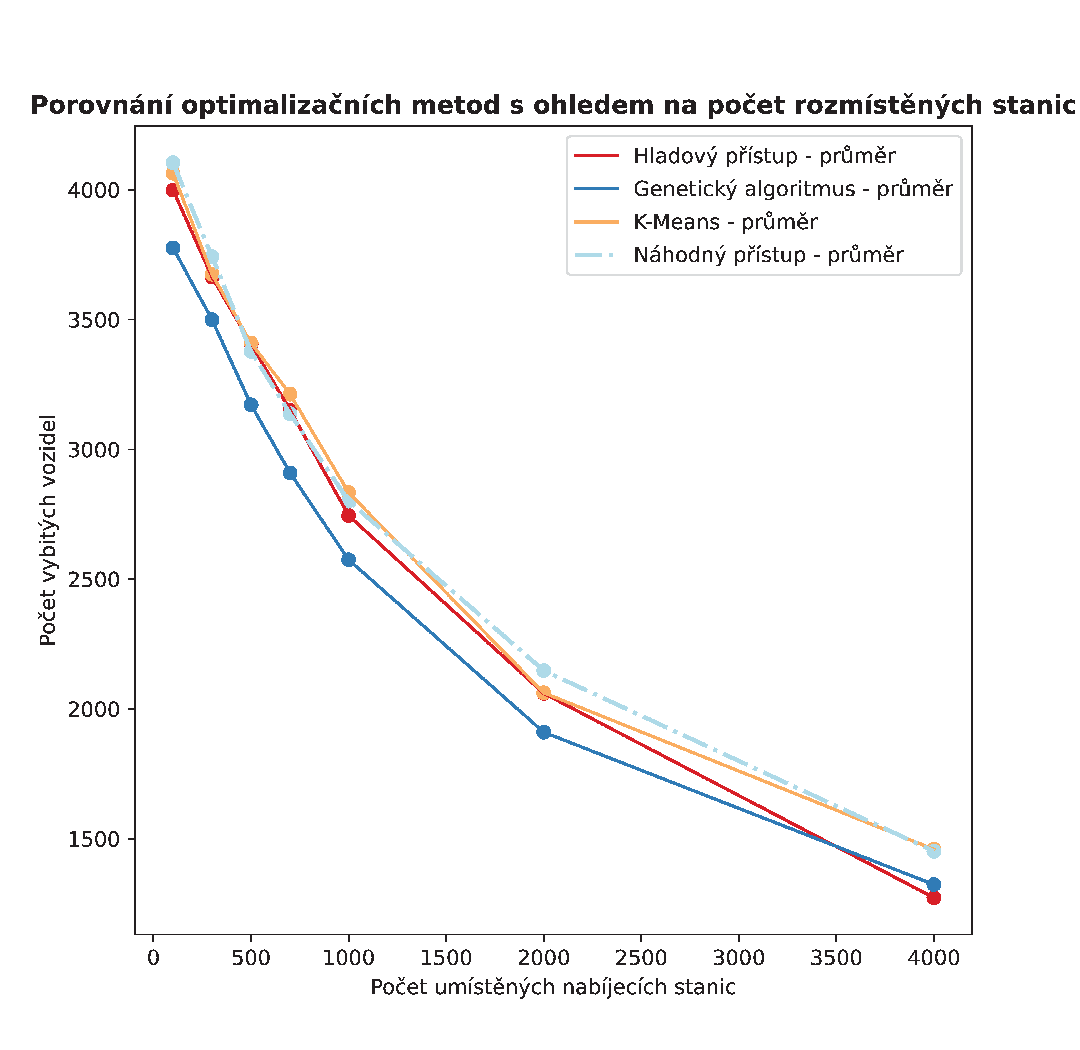
\includegraphics[width=1\linewidth]{img/all.pdf}
    \caption{Porovnání různých optimalizačních metod. Optimalizační metody barevně
    rozlišujeme. Čárové grafy popisují průměrné hodnoty počtu vybitých vozidel při
    daném počtu nabíjecích stanic umístěných v dopravní síti. 
    Čerchovaný čárový graf značí výsledky náhodného přístupu.}
    \label{fig:porovnani_optimalizaci_all}
\end{figure}


\begin{figure}
    \centering
    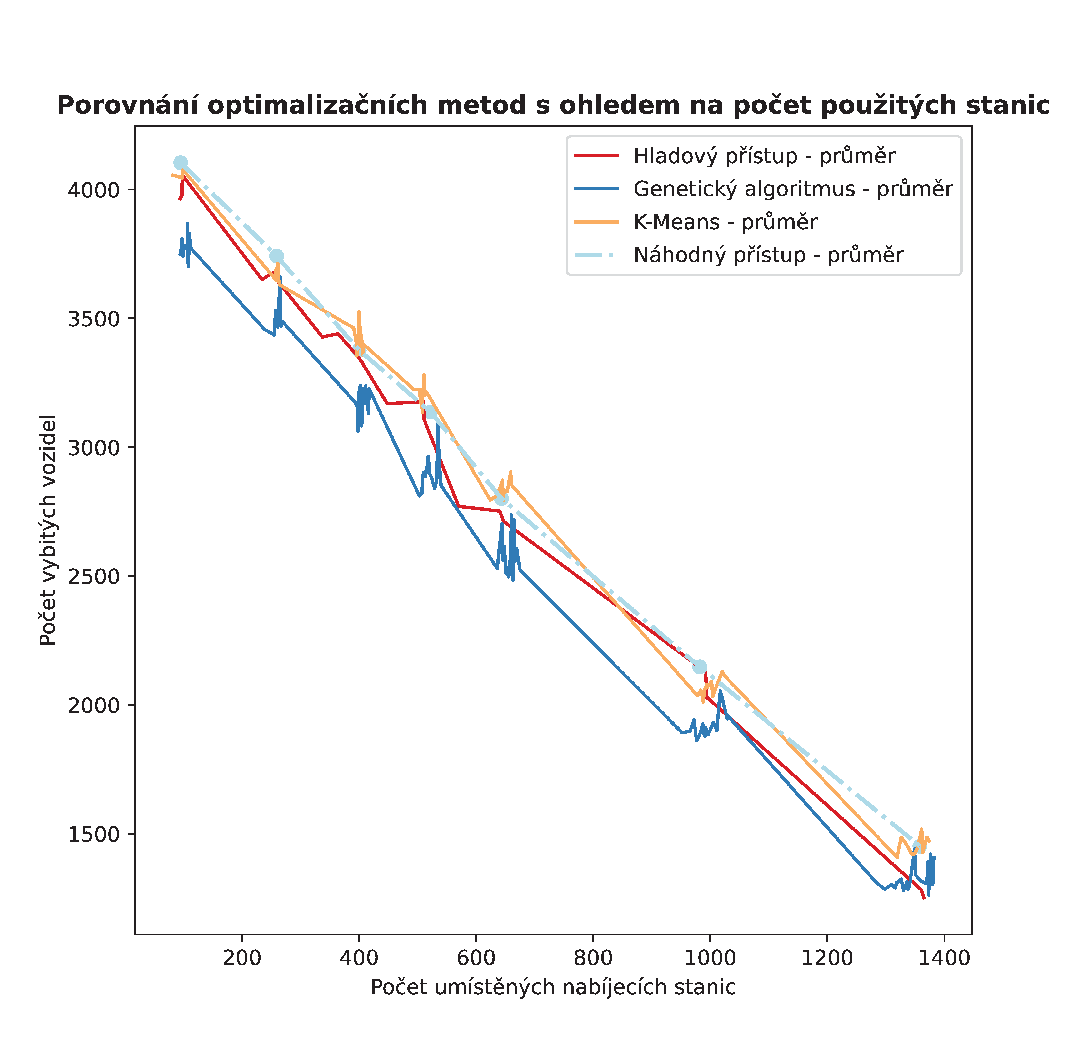
\includegraphics[width=1\linewidth]{img/used.pdf}
    \caption{Porovnání různých optimalizačních metod. Optimalizační metody barevně
    rozlišujeme. Čárové grafy popisují průměrné hodnoty počtu vybitých vozidel při
    daném počtu aspoň jednou použitých nabíjecích stanic v dopravní síti. 
    Čerchovaný čárový graf značí výsledky náhodného přístupu.}
    \label{fig:porovnani_optimalizaci_used}
\end{figure}
% 
\ifEN
\chapwithtoc{Bibliography}
\else
\chapwithtoc{Seznam použité literatury}
\fi

\printbibliography[heading=none]


% \appendix
% \chapter{Uživatelská dokumentace}
\label{chap:uzivatelska_dokumentace}

Hlavním cílem programu je na zvolené reprezentaci mapy opakovaně simulovat 
dopravní síť a na základě této simulace optimalizovat rozmístění nabíjecích
stanic s pomocí různých optimalizačních algoritmů. Po ukončení optimalizace
vypíše zvolené relevantní informace o jednotlivých simulacích pro následnou 
analýzu optimalizačních metod. Program také nabízí nastavitelnost široké škály 
parametrů simulátoru dopravy i optimalizačních  metod pro detailnější analýzu.


\section{Příprava před spuštěním}
Rozlišujeme více variant spuštění programu podle OS, který používáme.

Pokud pracujeme v OS \textbf{Windows 10}, pak můžeme použít již předkompilovaný 
program, jenž je součástí přílohy. V tomto případě můžeme program rovnou spustit.
Předkompilovaný spustitelný se nachází v adresáři:

\begin{verbatim}
    Win_executable/
\end{verbatim}

V tomto adresáři se nachází spustitelný program, adresář s předpřipravenou
reprezentací mapy a další pomocné soubory pro správné fungování programu.
Název spustitelného programu je:

\begin{verbatim}
    Traffic_Simulator.exe 
\end{verbatim}

\subsection{Sestavení programu}
Pokud chceme program sestavit, pak je potřeba postupovat v následujících krocích.

\subsubsection{Sestavení pro OS Linux}

Pro sestavení programu v OS Linux potřebujeme
\texttt{CMake 3.11}\footnote{\url{https://cmake.org/}}, 
nebo vyšší (doporučujeme verzi \texttt{3.14+}), překladač podporující \texttt{C++11},
knihovnu \texttt{Boost}\footnote{\url{https://www.boost.org/}} a
Git\footnote{\url{https://git-scm.com/}}.

Nejprve se přesuneme do adresáře s požadovanými zdrojovými kódy.
\begin{verbatim}
    cd source_code/Traffic_Simulator_cmake
\end{verbatim}

Pro konfiguraci spustíme příkaz (přidáme ještě možnost \texttt{-GNinja}, 
pokud používáme Ninja\footnote{\url{https://ninja-build.org/}}).
\begin{verbatim}
    cmake -S . -B build
\end{verbatim}

Pro sestavení programu spustíme příkaz:
\begin{verbatim}
    cmake --build build
\end{verbatim}

Výsledný spustitelný program pak nalezneme:
\begin{verbatim}
    build/apps/Traffic_Simulator
\end{verbatim}

\subsubsection{Sestavení pro OS Windows 10}
Pro sestavení programu v OS Windows 10 potřebujeme překladač podporující 
\texttt{C++11}, Visual Studio 2019\footnote{https://visualstudio.microsoft.com/cs/},
Git a \texttt{vcpkg}\footnote{\url{https://github.com/microsoft/vcpkg}}.

Nejprve se přesuneme do adresáře, kde je uložen nástroj \texttt{vcpkg} a 
nainstalujeme knihovnu Boost.
\begin{verbatim}
    cd $(Absolute_Path_To_vcpkg_Directory)

    .\vcpkg\vcpkg install boost
    .\vcpkg\vcpkg integrate install
\end{verbatim}

Následně se přesuneme do adresáře naší práce a zde do adresáře:

\begin{verbatim}
    cd source_code\Traffic_Simulator_VS
\end{verbatim}
 
Zde nalezenem soubor:
\begin{verbatim}
    Traffic_Simulator.sln
\end{verbatim}

Ten otevřeme v programu Visual Studio 2019, ve kterém projekt sestavíme.

\section{Poznámka k příkladům}
V následujícím textu popisujeme příklady použití programu v OS Linux.
Pokud pracujeme v OS Windows, pak program spouštíme následujícím příkazem
(se zvolenými parametry (viz. \cref{subsec:parametry_programu})):

\begin{verbatim}
    .\Traffic_Simulator.exe
\end{verbatim}

Pokud pracujeme s předpřipravenou mapou z adresáře:
\begin{verbatim}
    preprocesed\_maps
\end{verbatim}

Pak musíme pro fungování příkazů v příkladech, zkopírovat tento adresář do 
adresáře se spustitelným souborem programu. Pokud pracujeme s již
předkompilovaným programem v OS Windows, pak tato operace není nutná.

\section{Formát souborů reprezentujících mapu}
\label{sec:soubor_mapy}

Pro správné fungování programu je potřeba při každém spuštění načíst reprezentaci
mapy (\cref{sec:dopravni_sit}).
Ta je rozdělena do 3 souborů a informace v nich zapsané si nesmějí 
navzájem odporovat. Tyto 3 soubory jsou načítany v pořadí: soubor s reprezentací
křižovatek, soubor s reprezentací silnic a soubor s reprezentací měst.
Vzhledem k obvykle velké objemnosti dat reprezentující dopravní síť je 
doporučeno při přípravě vstupních souborů postupovat podle
kroků, jež popisuje \cref{chap:priprava_mapy}, s pomocí přiložených programů
v adresáři \texttt{map\_preprocessing} práce (viz. \cref{chap:prilohy}).

Pokud chce uživatel pracovat pouze s námi připravenou mapou České republiky, 
jenž podrobněji popisuje \cref{chap:priprava_mapy}, je v adresáři
\texttt{preprocesed\_maps} dodána reprezentace již připravené mapy.
Struktura adresáře je:

\begin{verbatim}
./prepared_graph/
    cities.txt
    combined_nodes.txt
    edges.txt
    prepared_combined_nodes.txt
    prepared_edges.txt
\end{verbatim}

V souborech výše jsou zapsány po řadě, reprezentace měst, reprezentace křižovatek,
reprezentace hran a v souborech s předponou \texttt{prepared\_} je uložena 
předpřipravená reprezentace mapy (bez křižovatek stupně 2) se stejnou reprezentací,
jako v neupravené variantě (reprezentace měst se předpřípravou nemění).

Formát všech vstupních souborů je strukturován po řádcích. V každém souboru
je vždy ignorován první řádek, jehož účelem je popis formátu vstupních dat 
jednotlivých řádků pro každý vstupní soubor. S ohledem na 
přehlednost vstupních dat je doporučeno tento formát vždy dodržovat.
Ve zbytku souboru je postupně na každém řádku reprezentován specifický objekt
mapy, který je určen daným typem souboru. Jakékoli nedodržení formátu
vstupních souborů vede s vysokou pravděpodobností k selhání načítání dat a
není tak umožněna další práce s programem.


\subsection{Soubor reprezentující křižovatky}
\label{subsec:reprezentace_krizovatky}

Předpokládaná hlavička (1. řádek) souboru je:
\begin{Verbatim}
    node_id latitude longitude city_id distance_km 
\end{Verbatim}

Každý řádek, kromě prvního řádku, reprezentuje právě jednu kžižovatku (\cref{def:krizovatka}).
Požadujeme, aby na každém řádku bylo uloženo pět hodnot oddělených mezerou, které 
reprezentují po řadě: identifikační číslo (ozn. ID) křižovatky, zeměpisnou šířku,
v níž se křižovatka nachází, zeměpisnou délku, v níž se křižovatka nachází,
ID města, do něhož křižovatka náleží, a vzdálenost křižovatky od centra tohoto města.

Pro správnou funkci programu je potřeba, aby ID křižovatek byla celá nezáporná 
čísla a aby křižovatky byly v souboru seřazeny vzestupně bez vynechaných hodnot ID.
Tedy pokud např. v souboru existuje vrchol s ID 6, musí být předem definovány
vrcholy s ID v rozmezí od 1 do 5. Dále požadujeme, aby ID křižovatek byly unikátní.
Zeměpisná šířka, zeměpisná délka i vzdálenost města jsou reprezentovány 
desetinným číslem s desetinnou tečkou. ID města je reprezentováno nezáporným
celým číslem, jež musí být zadefinováno v souboru reprezentující města 
(\cref{subsec:reprezentace_mesta}).


Příklad formátu vstupního souboru, jenž reprezentuje křižovatky:
\begin{Verbatim}
    node_id latitude longitude city_id distance_km
    0 50.0354962 14.4080276 1 5.855519633308941 
    1 50.0352373 14.4080465 2 5.883717272182215 
    2 50.0350876 14.4080758 0 5.8998150943334124
    3 50.035876 14.4080352 0 5.8898140943334124
\end{Verbatim}


\subsection{Soubor reprezentující silnice}

Předpokládaná hlavička (1. řádek) souboru je:
\begin{Verbatim}
new_node_id_1 new_node_id_2 length road_type
\end{Verbatim}
Každý řádek, kromě prvního řádku, reprezentuje právě jednu silnici (\cref{def:silnice})
dopravní sítě. Požadujeme, aby na každém řádku byly uloženy čtyři hodnoty oddělené
mezerou reprezentující: ID první křižovatky definující silnici, ID druhé
křižovatky definující silnici, délka silnice a typ silnice.
Předpokládáme, že ID křižovatek jsou v odpovídajícím formátu, 
který je popsán v části pro reprezentaci křižovatek (\cref{subsec:reprezentace_krizovatky})
a zároveň, že křižovatka s ID ze vstupu byla definována a načtena ze souboru 
pro reprezentaci křižovatek.
Délka silnice je reprezentována desetinným číslem s desetinnou tečkou.
\Cref{tab:typy_silnice} vypisuje všechny typy silnice a jejich reprezentaci pro
vstupní soubor.

\begin{table}
\centering\footnotesize\sf
\begin{tabular}{ll}
\toprule
Reprezentace & Popis \\
\midrule
\texttt{m} & dálnice  \\
\texttt{t} & silnice pro motorová vozidla \\
\texttt{p} & silnice 1. třídy nebo  \\
\texttt{o} & jiný druh silnice \\
\bottomrule
\end{tabular}
\caption{Výpis všech variant druhů silnice.}
\label{tab:typy_silnice}
\end{table}
    

Příklad formátu vstupního souboru, jenž reprezentuje silnice:
\begin{Verbatim}
new_node_id_1 new_node_id_2 length road_type
0 1 28.82 t 
1 2 16.777 p
2 3 17.303 m
\end{Verbatim}


\subsection{Soubor reprezentující města}
\label{subsec:reprezentace_mesta}

Předpokládaná hlavička (1. řádek) souboru je:
\begin{Verbatim}
city_id lat lon population
\end{Verbatim}
Každý řádek, kromě 1. řádku, reprezentuje právě 1 město (\cref{def:mesto}).
Požadujeme, aby na každém řádku byly uloženy 4 hodnoty oddělené mezerou reprezentující:
ID města, zeměpisnou šířku, v níž se nachází střed města, zeměpisnou délku, v 
níž se nachází střed města, a počet obyvatel města.
Požadujeme, aby ID města bylo nezáporné celé číslo. Pro zajištění správného 
fungování programu je doporučeno reprezenovat města v souboru v rostoucím
pořadí podle ID města bez opakování a bez vynechaných ID. Tato podmínka 
však není na rozdíl od reprezentace křižovatek nutná.
Zeměpisná šířka a délka jsou reprezentovány desetinným číslem s desetinnou 
tečkou. Populace města je reprezentována nezáporným celým číslem.

Příklad formátu vstupního souboru, jenž reprezentuje  města:
\begin{Verbatim}
city_id lat lon population
0 49.39606475830078 15.590306282043457 51216 
1 49.70147705078125 17.07569122314453 7516 
2 51.02574920654297 15.061005592346191 4259 
\end{Verbatim}


\subsection{Výstupní soubory}

Program také umožňuje zápis aktuálně načtené mapy do souborů ve vstupním formátu
simulátoru. Tato funkcionalita je především užitečná, pokud je předpříprava
původní mapy výpočetně náročná (odstraňování vrcholů stupně 2 nebo 
sjednocování komponent souvislosti). V takovém případě můžeme předpřipravenou
mapu uložit do formátu určeného pro načítání mapy a při opakovaném výpočtu
přeskočit předpřípravu dat a rovnou spustit požadovaný výpočet.


\section{Ovládání programu}

Uživatel interaguje s programem pouze při jeho spuštění, kdy je potřeba
zvolit příslušnou optimalizační metodu, její parametry a parametry simulace.
Před spuštěním programu je potřeba připravit soubory s korektní 
reprezentací mapy (\cref{sec:soubor_mapy}) a specifikovat 
cestu k těmto souborům.


\subsection{Parametry programu}
\label{subsec:parametry_programu}
Při spuštění programu zadáváme do terminálu parametry, kterými specifikujeme
požadované chování simulátoru. Tyto parametry zapisujeme ve formě přepínačů za
příkaz spouštějící program. Tyto přepínače popisujeme v tabulkách rozdělených
podle jejich funkce.
\Cref{tab:prepinace_pomocne} popisuje pomocné přepínače programu, 
\cref{tab:prepinace_soubory} popisuje přepínače pro specifikování vstupních a 
výstupních souborů, \cref{tab:prepinace_simulace} popisuje přepínače pro volbu
parametrů simulace, \cref{tab:prepinace_optimalizace} popisuje přepínače pro 
volbu obecných vlastností typických pro všechny optimalizační metody,
\cref{tab:prepinace_greedy} popisuje přepínače pro volbu parametrů hladové optimalizace,
\cref{tab:prepinace_genetic}, popisuje přepínače pro volbu parametrů optimalizace genetickým
algoritmem, \cref{tab:prepinace_kmeans} popisuje přepínače pro volbu parametrů optimalizace
pomocí algoritmu k-means a \cref{tab:prepinace_volba_optim} popisuje přepínače pro volbu
optimalizační metody.

\begin{table}
\centering\footnotesize\sf
\begin{tabular}{p{0.15\linewidth} p{0.75\linewidth}}
\toprule
Příkaz & Popis funkce \\
\midrule
\texttt{help} & Vypíše všechny možnosti parametrů programu. \\
\texttt{logs} & Program bude vypisovat podrobné informace o průběhu simulace 
(pro ladění progamu). \\
\bottomrule
\end{tabular}
\caption{Popis pomocných přepínačů v programu.}
\label{tab:prepinace_pomocne}
\end{table}


\begin{table}
\centering\footnotesize\sf
\begin{tabular}{p{0.30\linewidth} p{0.6\linewidth}}
\toprule
Příkaz & Popis funkce \\
\midrule
\texttt{nodeCityFile arg} & Cesta k vstupnímu souboru s reprezentací křižovatek. 
V případě nespecifikované hodnoty je zvolena cesta:
\texttt{prepared\_graph/combined\_nodes.txt} \\
\texttt{edgesFile arg} & Cesta k vstupnímu souboru s reprezentací silnic.
V případě nespecifikované hodnoty je zvolena cesta:
\texttt{prepared\_graph/edges.txt} \\
\texttt{citiesFile arg} & Cesta k vstupnímu souboru s reprezentací měst. 
V případě nespecifikované hodnoty je zvolena cesta:
\texttt{prepared\_graph/cities.txt} \\
\texttt{addedEdgesFile arg} & Cesta k výstupnímu souboru pro uložení reprezentace 
přidaných hran pro vytvoření souvislého grafu. 
V případě nespecikované hodnoty je zvolena cesta:
\texttt{prepared\_graph/added\_edges.txt} \\
\texttt{preparedNodesFile arg} & Cesta k výstupnímu souboru pro uložení reprezentace
vrcholů upraveného grafu po eliminaci vrcholů stupně 2.
V případě nespecikované hodnoty je zvolena cesta:
\texttt{prepared\_graph/prepared\_combined\_nodes.txt} \\
\texttt{preparedEdgesFile arg} & Cesta k výstměupnímu souboru pro uložení reprezentace
hran upraveného grafu po eliminaci vrcholů stupně 2 
V případě nespecikované hodnoty je zvolena cesta:
\texttt{prepared\_graph/prepared\_edges.txt}\\
\texttt{savePrepared} & Parametr specifikující, zda uložit předpřipravenou 
reprezentaci mapy. \\
\bottomrule
\end{tabular}
\caption{Popis přepínačů pro specifikování vstupních a výstupních souborů.}
\label{tab:prepinace_soubory}
\end{table}


\begin{table}
\centering\footnotesize\sf
\begin{tabular}{p{0.43\linewidth} p{0.5\linewidth}}
\toprule
Příkaz & Popis funkce \\
\midrule
\texttt{simulationTime arg} & Doba simulace v minutách. \\
\texttt{segmentLength arg} & Délka hrany grafu v kilometrech. \\
\texttt{numClosestStations arg} & Počet nabíjecích stanic, které jsou zvažovány 
    při plánování cesty vozidla na nabíjecí stanici. \\
\texttt{carConsumption} & Spotřeba baterie vozidla v procentech kapacity za minutu. \\
\texttt{numStations arg} & Celkový počet nabíjecích stanic v simulaci. \\
\texttt{stationCapacity arg} & Počet nabíjecích slotů na každé stanici. \\
\texttt{exponentialLambdaCities arg} & Parametr pro generování cílového města vozidla.
    Hodnota je rovna $\frac{1}{d}$, kde $d$ je střední hodnota vzdálenosti 
    cílového města od startu v kilometrech. \\
\texttt{exponentialLambdaDepartures arg} & Parametr pro generování času výjezdu
    následujícího vozidla. Hodnota je rovna $\frac{1}{t}$, kde $t$ je střední 
    hodnota času následujícího výjezdu vozidla v minutách. \\
\texttt{endCityRatio arg} & Parametr specifikující důležitost vzdálenosti cílového
    města vůči počtu obyvatel při generování cílového města 
    (viz. \cref{def:pravdepodobnost_ciloveho_mesta}). Pokud $<1$, pak je
    počet obyvatel důležitější. Pokud $=1$, pak jsou oba parametry stejně důležité.
    Pokud $>1$, pak je důležitější vzdálenost města. \\
\texttt{batteryTresholdLambda arg} & Hodnota $\frac{1}{b}$, kde $b$ je střední 
    hodnota hladiny baterie specifikující, o kolik průměrně převyšuje hladina baterie v době
    rozhodnování nejnižší možnou hranici pro rozhodnutí, zda jet nabíjet, v moment rozhodnutí
    (viz. \cref{subsec:zajizdeni_na_nabijecku}). \\
\texttt{carBatteryMean arg} & Střední hodnota počáteční hladiny baterie. \\
\texttt{carBatteryDeviation arg} & Směrodatná odchylka počáteční hladiny baterie vozidla. \\
\texttt{carStartBatteryBottomLimit arg} & Minimální hladina baterie vozidla při výjezdu. \\
\texttt{chargingTreshold arg} & Nejnižší možná hladina baterie pro rozhodnutí,
    zda vyrazit na nabíjecí stanici (viz. \cref{subsec:zajizdeni_na_nabijecku}). \\
\texttt{notChargingTreshold arg} & Nejvyšší hladina pro rozhodnutí, zda vyrazit na 
    nabíjecí stanici (viz. \cref{subsec:zajizdeni_na_nabijecku}). \\
\texttt{batteryTolerance arg} & Nejnižší možná očekávaná hladina baterie v cíli, 
    kdy se při rozhodování, rozhodnout nezajet na nabíjecí stanici 
    (viz. \cref{subsec:zajizdeni_na_nabijecku}). \\
\texttt{carVelocity arg} & Průměrná rychlost všech vozidel v kilometrech za minutu. \\
\texttt{chargingWaitingTime arg} & Doba čekání na úplné nabití baterie v minutách.  \\
\texttt{meanChargingLevel arg} & Očekávaná střední hodnota hladiny baterie, jež
    je nabíjena na nabíjecích stanicích (pro odhad doby čekání nabíjení ve frontě).  \\
\bottomrule
\end{tabular}
\caption{Popis přepínačů pro specifikování parametrů simulátoru.}
\label{tab:prepinace_simulace}
\end{table}


\begin{table}
\centering\footnotesize\sf
\begin{tabular}{p{0.42\linewidth} p{0.51\linewidth}}
\toprule
Příkaz & Popis funkce \\
\midrule
\texttt{lossDifferenceTreshold arg} & Minimální rozdíl ztrátové funkce pro 
pokračování v optimalizaci (pro vybrané optimalizační metody). \\
\texttt{stationNumberParameter arg} & Parametr počtu stanic při výpočtu ztrátové 
funkce (viz. \cref{sec:loss}).\\
\texttt{runDownParameter arg} & Parametr počtu vozidel, kterým se vybila baterie,
pro výpočet ztrátové funkce (viz. \cref{sec:loss}).\\
\texttt{durationParameter arg} & Parametr průměrné doby cestování v minutách pro
výpočet ztrátové funkce (viz. \cref{sec:loss}).\\
\texttt{batteryDifferenceParameter arg} & Parametr průměrného rozdílu hladin 
baterie pro výpočet ztrátové funkce (viz. \cref{sec:loss}).\\
\texttt{waitingTimesParameter arg} & Parametr průměrné čekací doby na nabíjecích
stanicích pro výpočet ztrátové funkce (viz. \cref{sec:loss}).\\
\bottomrule
\end{tabular}
\caption{Popis přepínačů pro specifikování obecných vlastností optimalizace.}
\label{tab:prepinace_optimalizace}
\end{table}


\begin{table}
\centering\footnotesize\sf
\begin{tabular}{p{0.35\linewidth} p{0.58\linewidth}}
\toprule
Příkaz & Popis funkce \\
\midrule
\texttt{greedyMaxIterations arg} & Maximální počet iterací algoritmu. \\
\texttt{greedyNumThrowAway arg} & Maximální rozdíl počtu stanic mezi iteracemi algoritmu. \\
\bottomrule
\end{tabular}
\caption{Popis přepínačů pro specifikování parametrů hladové optimalizace (viz. \cref{sec:greedy}).}
\label{tab:prepinace_greedy}
\end{table}


\begin{table}
\centering\footnotesize\sf
\begin{tabular}{p{0.52\linewidth} p{0.41\linewidth}}
\toprule
Příkaz & Popis funkce \\
\midrule
\texttt{geneticPopulatioSize arg} & Velikost populace. \\
\texttt{geneticNumGenerations arg} & Počet generací. \\
\texttt{geneticNumBestSelection arg} & Počet nejlepších jedinců pro zkopírování
    do následující generace. \\
\texttt{geneticTournamentSelectionTreshold arg} & Pravděpodobnost výběru lepšího
    jedince v turnajové selekci. \\
\texttt{geneticMutationTreshold arg} & Pravděpodobnost mutace nabíjecí stanice. \\
\texttt{geneticMemberSizeVariance arg} & Směrodatná odchylka rozdílu velikosti 
    nového jedince a jeho rodiče pro mutaci velikosti jedince. \\
\bottomrule
\end{tabular}
\caption{Popis přepínačů pro specifikování parametrů optimalizace genetickým algorimem
    (viz. \cref{sec:genetic_optim}).}
\label{tab:prepinace_genetic}
\end{table}


\begin{table}
\centering\footnotesize\sf
\begin{tabular}{p{0.46\linewidth} p{0.47\linewidth}}
\toprule
Příkaz & Popis funkce \\
\midrule
\texttt{kMeansNumIterationsOneRun arg} & Počet iterací jednoho běhu algorimu k-means. \\
\texttt{kMeansNumGenerations arg} & Počet generací modelů. \\
\bottomrule
\end{tabular}
\caption{Popis přepínačů pro specifikování parametrů optimalizace algoritmem k-means 
    (viz. \cref{sec:kmeans_optim}).}
\label{tab:prepinace_kmeans}
\end{table}


\begin{table}
\centering\footnotesize\sf
\begin{tabular}{p{0.17\linewidth} p{0.76\linewidth}}
\toprule
Příkaz & Popis funkce \\
\midrule
\texttt{randomModels} & Spustí pevný počet simulací na modelech s náhodně 
rozmístěnými nabíjecími stanicemi. \\
\texttt{greedy} & Spustí optimalizaci hladovým algoritmem. \\
\texttt{genetic} & Spustí optimalizaci genetickým algorimem. \\
\texttt{kMeans} & Spustí optimalizaci algoritmem K-Means. \\
\bottomrule
\end{tabular}
\caption{Popis přepínačů pro volbu optimalizační metody.}
\label{tab:prepinace_volba_optim}
\end{table}


\subsection{Příklad spouštění programu}
V této sekci uvádíme příklad spuštění programu se vstupními soubory. Po řadě pro
křižovatky, silnice a města s názvy:
\begin{Verbatim}
    prepared_graph/combined_nodes.txt
    prepared_graph/edges.txt
    prepared_graph/cities.txt
\end{Verbatim}

Dále uvádíme výstupní soubory. Po řadě pro soubor s nově přidanými hranami
po sloučení komponent souvislosti, pro reprezentaci vrcholů z předpřipraveného grafu 
a pro reprezentaci hran z předpřipraveného grafu:
\begin{Verbatim}
    prepared_graph/added_edges.txt, 
    prepared_graph/prepared_nodes_new.txt
    prepared_graph/prepared_edges_new.txt
\end{Verbatim}

Dále v tomto příkladě volíme čas simulace 100 minut, celkový počet stanic 300 a
počet generací genetického algoritmu 3. Nakonec specifikujeme, že chceme spustit 
optimalizaci genetickým algoritmem a uložit předpřipravenou mapu. Další parametry
jsou zvoleny automaticky, podle výchozí hodnoty nastavené v programu, kterou lze
dohledat příkazem:

\begin{Verbatim}
    ./Traffic_Simulator --help
\end{Verbatim}

Optimalizaci na parametrech popsaných výše spustíme příkazem:

\begin{Verbatim}
./Traffic_Simulator \
--nodeCityFile="prepared_graph/combined_nodes.txt" \
--edgesFile="prepared_graph/edges.txt" \
--citiesFile="prepared_graph/cities.txt" \
--addedEdgesFile="prepared_graph/added_edges.txt" \
--preparedNodesFile="prepared_graph/prepared_combined_nodes_new.txt" \
--preparedEdgesFile="prepared_graph/prepared_edges_new.txt" \
--simulationTime=100 \
--numStations=300 \
--geneticNumGenerations=3 \
--genetic \
--savePrepared
\end{Verbatim}


Pokud zvolíme vstupní soubory (křižovatek, silnic a města):

\begin{Verbatim}
    prepared_graph/prepared_combined_nodes.txt
    prepared_graph/prepared_edges.txt
    prepared_graph/cities.txt
\end{Verbatim}

Pokud nechceme ukládat předpřipravenou podobu grafu a parametry volíme stejně jako v minulém
případě, pak příkaz pro spuštění vypadá následovně:

\begin{Verbatim}
    ./Traffic_Simulator \
    --nodeCityFile="prepared_graph/prepared_combined_nodes.txt" \
    --edgesFile="prepared_graph/prepared_edges.txt" \
    --citiesFile="prepared_graph/cities.txt" \
    --simulationTime=100 \
    --numStations=300 \
    --geneticNumGenerations=3 \
    --genetic 
\end{Verbatim}


\section{Výstup programu}
První část výstupu programu je vždy výpis použitých parametrů. Část tohoto
výpisu může vypadat například následovně:

\begin{Verbatim}
Save prepared is: 0
Edges: prepared_graph/prepared_edges.txt
Node City: prepared_graph/prepared_combined_nodes.txt
Cities: prepared_graph/cities.txt
Simulation time: 1000
Length of the edge segment: 1
Number of closest stations: 10
Car consumtion: 0.001
Number of charging stations: 500
Capacity of the charging station: 1
...
\end{Verbatim}

Následuje část kontrolních zpráv o procesu eliminace křižovatek stupně 2. 
Program vždy po eliminaci 10000 křižovatek stupně 2 vypíše
informaci o úspěšném průběhu procesu eliminace křižovatek. 
Příklad tohoto výpisu může vypadat následovně:

\begin{Verbatim}
Iteration: 0 Vertices of degree 2 merged and deleted.
Iteration: 10000 Vertices of degree 2 merged and deleted.
Iteration: 20000 Vertices of degree 2 merged and deleted.
Iteration: 30000 Vertices of degree 2 merged and deleted.
Iteration: 40000 Vertices of degree 2 merged and deleted.
Iteration: 50000 Vertices of degree 2 merged and deleted.
Iteration: 60000 Vertices of degree 2 merged and deleted.
Iteration: 70000 Vertices of degree 2 merged and deleted.
Iteration: 80000 Vertices of degree 2 merged and deleted.
Iteration: 90000 Vertices of degree 2 merged and deleted.
Iteration DONE
\end{Verbatim}


Dále následuje posloupnost kontrolních zpráv o slučování komponent 
souvislosti, která je zakončena informací o spuštění zvolené optimalizační metody. 
Tato posloupnost může vypadat následovně (pro spuštění hladové optimalizační
metody):

\begin{Verbatim}
Total number of components: 16
Total number of components: 15
Total number of components: 14
Total number of components: 13
Total number of components: 12
Total number of components: 11
Total number of components: 10
Total number of components: 9
Total number of components: 8
Total number of components: 7
Total number of components: 6
Total number of components: 5
Total number of components: 4
Total number of components: 3
Total number of components: 2
Total number of components: 1
Running greedy algorithm.
\end{Verbatim}

Dále následuje výpis kontrolních zpráv o běhu simulace po každých 
10 odsimulovaných minutách, který je zakončen výsledky simulace a informací
o hodnotě ztrátové funkce. Tento výpis se periodicky opakuje pro každou
spuštěnou simulaci. 
Níže uvádíme příklad výpisu jednoho běhu simulace pro dobu 100 minut.

\begin{Verbatim}
Time 10 elapsed!
Time 20 elapsed!
Time 30 elapsed!
Time 40 elapsed!
Time 50 elapsed!
Time 60 elapsed!
Time 70 elapsed!
Time 80 elapsed!
Time 90 elapsed!
Time 100 elapsed!
Number of stations: 500
Number of run down batteries: 654393
Average traveling duration: 98.0642
Average battery difference between start and end: -0.345312
Average waiting times in charging station: 165.868
------------------------------------------------------
Model loss: 6.54896e+07
\end{Verbatim}

Po skončení všech simulací je program zakončen finálním výpisem informací o
modelu s nejmenší hodnotou ztrátové funkce, nebo v případě volby 
\texttt{randomModels} výpisem aritmetického průměru hodnot popisující vlastnosti simulace.

Speciálním případem je optimalizace za pomoci genetického algoritmu, kde jsou
před finálním výpisem vypsány hodnoty ztrátové funkce všech modelů použitých v průběhu
optimalizace. Část finálního výpisu genetického algoritmu před výpisem informací o nejlepším
modelu může pro 3 generace a velikost populace 3 vypadat následovně:

\begin{Verbatim}
Algorithm finished
Losses for the generation: 0
Loss: 7.58681e+07
Loss: 7.5309e+07
Loss: 7.55552e+07
Losses for the generation: 1
Loss: 7.44727e+07
Loss: 7.56497e+07
Loss: 7.46101e+07
Losses for the generation: 2
Loss: 7.55472e+07
Loss: 7.50069e+07
Loss: 7.56775e+07

Total best loss is: 7.44727e+07
\end{Verbatim}

Finální výpis nejlepších výsledků všech optimalizačních metod může vypadat následovně:

\begin{Verbatim}
Best model info:
------------------------------------------------------
Number of stations: 101
Number of run down batteries: 733511
Average traveling duration: 100.09
Average battery difference between start and end: -0.34632
Average waiting times in charging station: 203.302
------------------------------------------------------
Model loss: 7.33615e+07
\end{Verbatim}

Tento výpis nám říká, že v nejlepším modelu bylo použito $101$ nabíjecích stanic,
počet vozidel, kterým došla baterie je $733511$, průměrná doba cestování vozidla
v minutách je $100.09$, průměrný rozdíl počáteční a koncové hladiny baterie je 
$-0.34632$ (záporná hodnota znamená, že vozidlo dojelo do cíle s vyšší hladinou
baterie, než s jakou vyjíždělo), průměrný čas čekání vozidel na nabíjecích stanicí
než se dostanou na řadu je $203.302$ a nakonec hodnota ztrátové funkce modelu
je $7.33615e+07$.
% \chapter{Programátorská dokumentace}
\label{chap:prog_dok}

Účelem této části je především vysvětlit vzájemnou propojenost jednotlivých
tříd programu a vysvětlit jeho fungování v rámci celku. Podrobné informace o
konkrétních metodách jednotlivých tříd jsou popsány v podrobné dokumentaci
programu (viz. \cref{chap:prilohy}).


\section{Struktura programu}
Program je strukturován do vrstev tak, aby byla zajištěna jednoduchá práci s programem
na různých úrovni abstrakce. 

Uživatel pracuje pouze s nejabstraktnější vrstvou,
kterou je třída \texttt{Optimizer}, jež spravuje veškerou logiku spojenou s optimalizací.
Tato třída obaluje třídu \texttt{TimeTable}, jež je zodpovědná za správné fungování
diskrétní simulace a vytváři abstrakci pro třídu \texttt{TrafficSimulator}. Třída
\texttt{TrafficSimulator} je zodpovědná především za generování
událostí simulace (např. následující výjezd vozidla, odkud vozidlo vyjede a 
kam směřuje apod.) a propojení všech objektů simulace. Důležitým aspektem této 
vrsty je správa načítání mapy. Třída spravuje objekty třídy \texttt{MapReader}
a \texttt{GraphAdjuster} zodpovědné za správné předzpracování mapy. Dále je zodpovědná
za veškeré objekty abstraktní třídy \texttt{Vehicle}, které reprezentují vozidla v 
simulaci. V neposlední řadě také vytváří abstrakci pro třídy \texttt{Map}, která 
reprezentuje nejnižší vrstvu programu. Třída
\texttt{Map} je zodpovědná za veškeré grafové operace a veškeré operace pracující s 
reálnou zeměpisnou pozicí. Její součástí je objekt knihovny \texttt{boost}
s názvem \texttt{graph\_} reprezentující graf silniční sítě. Dále třída shlukuje 
informace o nabíjecích stanicích (reprezentované pomocí třídy \texttt{ChargingStation})
a městech náležících do simulované oblasti. 

Součástí programu je také řada dalších tříd pokrývající pomocné operace programu.
Některé z nich jsme již zmínili (\texttt{MapReader}, \texttt{GraphAdjuster}, 
\texttt{Vehicle}, 
\texttt{ChargingStation}). Za zmínku stojí ještě třídy \texttt{Car}, jež je potomkem třídy
\texttt{Vehicle} reprezentující typ vozidla "auto" (viz. \cref{subsec:druhy_vozidel}),
\texttt{Edge}, která pokrývá funkcionalitu a vlastnosti silnice v mapě (viz. \cref{def:silnice})
a \texttt{Node}, jež plní funkci křižovatek na mapě (viz. \cref{def:krizovatka}).
Zbylé třídy slouží především pro shlukování souvisejících informací 
(parametry simulátoru, optimalizací, vlastnosti nabíjecích stanic, modelu apod.).

Jedinou vyjímkou, jež není součástí struktury výše je část pracující s 
parametry programu, jež je realizována pomocí knihovny \texttt{boost}. Přesněji pomocí
funkcionalit z \texttt{program\_options}.


\section{Třída Optimizer}

Třída \texttt{Optimizer} je hlavní třídou celého programu, která na základě 
uživatelských vstupů spouští a realizuje zvolenou optimalizaci. Vytváří 
abstrakci nad třídou \texttt{TimeTable}, jež používáme pro spouštění simulací. 
Do rozhraní třídy náleží metody spouštějící optimalizační algoritmy:

\begin{verbatim}
    GreedyAlgorithm
    GeneticAlgorithm
    KMeansAlgorithm
\end{verbatim}

Metoda, jež počítá ztrátovou funkci modelu po uběhnutí simulace:
\begin{verbatim}
    ModelLoss
\end{verbatim}

A metoda, která opakovaně simuluje provoz na náhodně vygenerovaném modelu:
\begin{verbatim}
    RunMultipleSimulations
\end{verbatim}

Tato metoda slouží pro analýzu optimalizačních metod pro porovnání metod s 
náhodným přístupem. \Cref{chap:optim} nabízí podrobnější popis jednotlivých 
optimalizačních metod a ztrátové funkce. Dále třída obsahuje řadu privátních 
metod zajišťujících správnou funkčnost hlavních metod popsaných výše. Více informacím
je specifikováno v podrobné dokumentaci (viz. \cref{chap:prilohy}).

\section{Třída TimeTable}

Třída \texttt{TimeTable} je třída zodpovědná za správné fungování diskrétní
simulace. Vytváří abstrakci třídy \texttt{TrafficSimulator} a slouží jako rozhraní pro
zisk informací o vlastnostech simulace (pro analýzu optimalizačních metod). 
Do jejího rozhraní náleží především funkce spravující diskrétní simulaci.
Další skupinou metod této třídy jsou metody s předponou \texttt{Get}, 
s jejíž pomocí jsme schopni získat relevantní informace o simulaci.
Jediná metoda, jež nenáleží do zmíněných skupin je \texttt{LoadMap}. Ta slouží
jako zprostředkovatel žádosti o načtení mapy a spouští příslušné
metody ve třídě \texttt{TrafficSimulator}.

\Cref{chap:prubeh_simulace} nabízí podrobnější popis fungování diskrétní
simulace.


\section{Třída TrafficSimulator}

Třídu \texttt{TrafficSimulator} lze považovat za jádro celého simulátoru, jejíž funkce
je spravovat objekty simulace. V rámci simulace je zodpovědná především za
generování náhodných jevů (pozice nabíjecích stanic, generování vozidel, doby 
následující akce apod.) (viz. \cref{subsec:generovani_vozidel}), 
jež je zastoupeno metodami s předponou \texttt{Generate}. Pomocí této třídy jsou v simulaci
spravovány objekty vozidel (potomci třídy \texttt{Vehicle}). Zásadní vlastností této třídy
je vytváření rozhraní pro práci s třídou \texttt{Map}, jež pokrývá veškeré grafové 
operace programu. S třídou \texttt{Map} také úzce souvisí třídy 
\texttt{MapReader} a \texttt{GraphAdjuster}, sloužící pro načtení a předpřípravu
uživatelské reprezentace mapy do formátu, jenž je uložen
ve třídě \texttt{Map}. \Cref{sec:soubor_mapy} podrobně popisuje formát vstupních souborů.


\section{Třída Map}

Třída \texttt{Map} je technicky nejkomplexnější část programu. Slouží
jako rozhraní pro veškeré grafové operace a operace, jež pracují s reálnou
geografickou pozicí na mapě. Graf dopravní sítě je reprezentován pomocí 
příslušných objektů grafové části knihovny \texttt{boost}. Dále jednotlivé křižovatky 
(\cref{def:krizovatka}) a silnice (\cref{def:silnice}) jsou navíc reprezentovány 
vlastními objekty třídy \texttt{Node} (křižovatky) a \texttt{Edge} (silnice). 
Třída také sdružuje všechny nabíjecí stanice (\cref{def:nabijeci_stanice}) vyskytující 
se v mapě (reprezentovány třídou \texttt{ChargingStation}) a informace o rozmístění a 
populaci měst (\cref{def:mesto}) v simulované oblasti.

Třída obsahuje metody pro spravování podoby grafu, informací o nabíjecích 
stanicích a městech. Tyto funkcionality pokrývají metody s předponou \texttt{Add} a 
\texttt{Set}. Dále jsou zde metody pro získávání informací o objektech mapy začínající
příponou \texttt{Get} a \texttt{Exist} a metody přímo související s diskrétní simulací a 
optimalizací (\texttt{ResetSimulation} a \texttt{SimulateVehiclePassedThroughEdge}). Poslední
skupinou metod jsou nejkomplexnější operace třídy pracující s grafem, či mapou.


\subsection{Operace na mapě}

S ohledem na řešený problém je velmi důležitým aspektem návrhu hledání 
nejkratších cest. Program umí pracovat s 2 variantami algoritmu pro hledání
nejkratších cest v grafu. Těmi jsou Dijkstrův algoritmus, jenž je využívám
především pro hledání vzdáleností v grafu (např. v K-Means), a A-Star 
(\cref{sec:a_star}), jenž je používám v diskrétní simulaci pro hledání 
nejvýhodnější cesty vozidla (viz. \cref{subsec:hledani_trasy}).
Jako heuristika algoritmu A-Star je zvolena reálná geografická vzdálenost
mezi křižovatkami, která je spočítána pomocí příslušných vztahů pro výpočet
sférické vzdálenosti (viz. \cref{sect:zem_souradnice}). 

Dijkstrův algoritmus, algoritmus A-Star a výpočet sférické vzdálenosti je realizován
pomocí metod (ve stejném pořadí, jak jsou vypsány):

\begin{Verbatim}
    DijkstraFindDistances
    FindShortestPath
    ComputeSphericalDistance
\end{Verbatim}

Speciální metodou související s výpočtem nejkratší cesty v grafu je:

\begin{Verbatim}
    FindVehiclePath
\end{Verbatim}

Ta hledá nejkratší cestu mezi vrcholy, ale bere také v úvahu potřebu návštěvy nabíjecí
stanice, z níž vybere heuristicky tu nejvhodnější (viz. \cref{subsec:zajizdeni_na_nabijecku}).

Další metodou pracující s grafy je metoda pro hledání komponent souvislosti, 
využívaná v předpřípravě mapy pro simulaci.

\begin{Verbatim}
    TestComponents
\end{Verbatim}

Třída také obsahuje metodu hledající nejbližšího města od křižovatek a nejbližší
nabíjecí stanice od středů měst:

\begin{Verbatim}
    FindCityNodes
    FindCitiesNearestChargingStations
\end{Verbatim}


\section{Třídy objektů mapy}

Mezi třídy reprezentující objekty na mapě patří reprezentace křižovatek (\texttt{Node}),
silnic (\texttt{Edge}) a nabíjecích stanic (\texttt{ChargingStation}). 
Tyto třídy slouží především pro udržování informací o vlastnostech objektů,
obsahují však také jednoduchou logickou vrstvu pokrývající především správnou 
inicializaci, či aktualizaci informací v průběhu simulace. Třída \texttt{ChargingStation}
také pokrývá logickou vrstvu související s nabíjením vozidel (spravuje čekání 
vozidel v řadě, doby nabíjení apod.).


\section{Třídy pro načítání a předpřípravu dat}

Reprezentaci mapy je potřeba na začátku programu načíst z předpřipraveného 
formátu (viz. \cref{sec:soubor_mapy}) a řádně zpracovat do podoby s níž bude
simulátor dále pracovat (\cref{def:graf_site}). K tomuto
účelu slouží třídy \texttt{MapReader} a \texttt{GraphAdjuster}.

\subsection{Třída MapReader}
Třída \texttt{MapReader} převádí vstupní reprezentaci dat do požadovaného formátu
pomocí metod s předponou \texttt{Load}. Nejdůležitější metodou tohoto typu je metoda
\texttt{LoadMap}, jež načte veškeré potřebné informace a provede také předpřípravu 
mapy pro správné fungování simulátoru a zlepšení efektivity. Zmíněné úpravy
provádí s pomocí třídy \texttt{GraphAdjuster}. Dalším charakteristickou vlastností třídy
\texttt{MapReader} je možnost uložení aktuální reprezentace mapy (po předpřípravě mapy)
do souboru v požadovaném vstupním formátu pro efektivnější opakované 
načítání mapy. Mezi tyto metody patří takové, jejichž přípona je \texttt{Write}.

Třída nabízí možnost načítat a zapisovat také reprezentaci všech nabíjecích
stanic modelu metodami:

\begin{verbatim}
    LoadChargingStations
    WriteStations
\end{verbatim}

\subsection{Třída GraphAdjuster}
Vzhledem k typicky velkému rozměru vstupních dat je pravděpodobné, že výsledná
reprezentace mapy nebude splňovat veškeré potřebné vlastnosti nutné k správnému
chování programu, či bude jejich reprezentace zbytečně neefektivní. 
Typickými příklady tohoto problému je rozpad grafu na více komponent souvislosti
či vznik vrcholů stupně 2. Podrobněji tuto problematiku popisuje \cref{chap:priprava_mapy}. 

Řešení těchto potíží zajisťuje třída \texttt{GraphAdjuster} úzce pracující s
třídou \texttt{MapReader}. Ta po načtení grafu zkontroluje zda je graf souvislý
a pokud není, pak jej převede do souvislé podoby 
(viz. \cref{subsubsec:souvislost_grafu}). Dále se také zbavuje veškerých vrcholů 
stupně 2, čímž výrazně zefektivňuje budoucí simulaci (viz. \cref{subsec:problemy_modelu}). 
Operace jsou realizovány metodami:

\begin{verbatim}
    MergeTwoComponents
    MergeDegreeTwoVertices
\end{verbatim}


\section{Třída Vehicle}

Třída \texttt{Vehicle} je třída zahrnující veškeré informace o daném vozidle (\cref{sec:vozidla}),
s jejíž pomocí je možné simulovat chování vozidel a příslušně tak upravovat simulátor.
Při návrhu této třídy byla snaha co nejobecněji vyjádřit chování vozidel 
různých druhů a jednotlivé druhy vozidel simulace následně reprezentovat třídou,
jež je potomkem \texttt{Vehicle}. V naší implementaci je zvolen pouze jeden typ vozidla a 
to typ \texttt{Car}, jehož specifickou vlastností je, že po dosažení cílové 
destinace vrací zpět do místa výjezdu (viz. \cref{subsec:druhy_vozidel}).

Metody třídy \texttt{Vehicle} slouží převážně k získávání informací o vozidle
jinými objekty (např. aktuální stav baterie, aktuální pozice, 
zda míří na nabíjecí stanici apod.), případně k nastavování stavových parametrů 
vozidel (míří na nabíjecí stanici, začalo čekat v řadě na nabíjení apod.)
Objekty třídy jsou také schopny spočítat čas a hladinu baterie po průjezdu
silnicí, dokonce i posloupnosti silnic (celé cesty). Tyto informace jsou důležité
především pro diskrétní simulaci (\cref{chap:prubeh_simulace}) a při rozhodování, 
zda je potřeba jet na nabíjecí stanici (\cref{subsec:zajizdeni_na_nabijecku}).
Zbylé metody slouží pro simulaci akcí vozidel. Je zde metoda pro aktualizaci
trasy vozidla a nabití vozidla:

\begin{verbatim}
    UpdateVehiclePath
    ChargeBattery
\end{verbatim}

Nakonec obsahuje třída i metody, jež řádně simulují průjezd vozidla po silnici. 
V tomto případě jsou naimplementovány 3 varianty, jež řeší všechny možné varianty
průjezdu vozidla (\cref{subsec:udalost_presunu}) po silnici 
(průjezd silnice, výjez z vniřku ven, cesta uvnitř silnice).


\section{Pomocné třídy}

Zbylé třídy implementace slouží především k zapouzdření souvisejících informací,
jako jsou například parametry simulátoru, optimalizací, informace o pozicích na mapě, 
shrnující popis modelu a mnoho dalších. Názvy zmíněných tříd jsou:

\begin{verbatim}
    SimulationParameters
    OptimizerParameters
    MapPosition
    ModelRepresentation
\end{verbatim}

Tyto třídy slouží především k uchovávání informací o specifických objektech a
zjednodušenou manipulaci s daty.


\section{Testy programu}

K programu jsou také dodány testy zvolených problematických funkcionalit a
především pak testy načítání uživatelských dat, která jsou často i s ohledem na 
objem vstupních dat zdrojem problémů. Jedná se o testy rozhraní Microsoft Unit
Testing Framework pro C++. Návod na spuštění testů je k dohledaní v \citep{corob-msft_2022}.
% \chapter{Přílohy práce}
\label{chap:prilohy}

K práci jsou přiloženy následující soubory.

Adresář se zdrojovými kódy a unit testy simulátoru dopravy:

\begin{verbatim}
    ./source_code/
        Traffic_Simulator_cmake/
        Traffic_Simulator_VS/
        README.md   
\end{verbatim}

Podrobná programátorská dokumentace:

\begin{verbatim}
    ./Traffic_Simulator_Manual.pdf
\end{verbatim}

Předpřipravené vstupní soubory simulátoru:

\begin{verbatim}
    ./prepared_graph/
        cities.txt
        combined_nodes.txt
        edges.txt
        prepared_combined_nodes.txt
        prepared_edges.txt
\end{verbatim}

Adresář s programem pro předpřípravu mapy:

\begin{verbatim}
    ./map_preprocessing/
        map_parser.py
        map_reader.py
        README.md
\end{verbatim}

Adresář s podrobnými výsledky simulací a výpis jejich parametrů:
\begin{verbatim}
    ./analysis_results/
        greedy_results/
        genetic_results/
        kmeans_results/
        random_results/
        simulation_parameters_results/
        README.md
\end{verbatim}

Adresář s programem pro přípravu úloh do Metacentra a analýzu výsledků experimentů:
\begin{verbatim}
    ./experiment_analysis/
        metacentrum_grid_search.py
\end{verbatim}


% if your attachments are complicated, describe them in a separate appendix
%\include{attachments}

\openright
\end{document}
